\documentclass[letterpaper]{article}

\usepackage{natbib,alifeconf}  %% The order is important

\usepackage{hyperref}

\usepackage{subcaption}

\usepackage{csquotes}

\usepackage{hhline}

\usepackage{amsmath}

\ifdefined\mydraft
\mydraft
\fi

\graphicspath{{img/}}

% *****************
%  Requirements:
% *****************
%
% - All pages sized consistently at 8.5 x 11 inches (US letter size).
% - PDF length <= 8 pages for full papers, <=2 pages for extended
%    abstracts.
% - Abstract length <= 250 words.
% - No visible crop marks.
% - Images at no greater than 300 dpi, scaled at 100%.
% - Embedded open type fonts only.
% - All layers flattened.
% - No attachments.
% - All desired links active in the files.

% Note that the PDF file must not exceed 5 MB if it is to be indexed
% by Google Scholar. Additional information about Google Scholar
% can be found here:
% http://www.google.com/intl/en/scholar/inclusion.html.


% If your system does not generate letter format documents by default,
% you can use the following workflow:
% latex example
% bibtex example
% latex example ; latex example
% dvips -o example.ps -t letterSize example.dvi
% ps2pdf example.ps example.pdf


% For pdflatex users:
% The alifeconf style file loads the "graphicx" package, and
% this may lead some users of pdflatex to experience problems.
% These can be fixed by editing the alifeconf.sty file to specify:
% \usepackage[pdftex]{graphicx}
%   instead of
% \usepackage{graphicx}.
% The PDF output generated by pdflatex should match the required
% specifications and obviously the dvips and ps2pdf steps become
% unnecessary.


% Note:  Some laser printers have a serious problem printing TeX
% output. The use of ps type I fonts should avoid this problem.


\title{TODO TITLE}
\author{Matthew Andres Moreno$^{1}$ \and Charles Ofria$^{1}$ \\
\mbox{}\\
$^1$BEACON Center, Michigan State University, East Lansing, MI 48824 \\
mmore500@msu.edu} % email of corresponding author

% For several authors from the same institution use the same number to
% refer to one address.
%
% If the names do not fit well on one line use
%         Author 1, Author 2 ... \\ {\Large\bf Author n} ...\\ ...
%
% If the title and author information do not fit in the area
% allocated, place \setlength\titlebox{<new height>} after the
% \documentclass line where <new height> is 2.25in



\begin{document}
\maketitle

\begin{abstract}

Constructing and studying artificial evolutionary systems that aim to indefinitely produce artifacts of continuing novelty and increasing complexity has proven --- and doubtlessly will continue on as  --- a rich vein for practical, scientific, philosophical, and artistic innovations.
Recent evidence has suggested existing computational artificial life systems might be meaningfully constrained by practical limitations on simulation scale.
Ackley's concept of indefinite scalability describes constraints on open-ended systems neccessary to incoroporate theoretically unbounded computational resources.
Here, we argue that as a bridge to true indefinite scalability, practical scalability should also be considered: how to design open-ended evolutionary systems to make effective use of existing, commercially-available parallel- and distributed-computing hardware.
%We review existing in , and open-ended systems should emphasize interaction between parallel hardware components.
We highlight log-time hardware interconnects as a potentialy fruitful tool for  practical scalability.
We prove several results about scaling relationships of per-component traffic load of small-world interaction networks embedded on computational mesh.
In some, but not all cases, log-time physical interconnects yield better asymptotic scaling behavior.
Then, we turn our attention to how digital evolution systems might be constructed to exploit of physical log-time interconnects.
We describe an extension to the DISHTINY digital multicellularity framework that  allows cells to establish long-distance cell-cell interconnects that, in implementation, could take advantage of log-time physical interconnects.
We examine two case studies of evolved strains, showing how adaptively exploit these interconnects.
\end{abstract}


\section{Introduction}

The challenge, and promise, of open-ended evolution has animated decades of inquiry and discussion within the artificial life community \citep{packard2019overview}.
The difficulty of devising models that reconstitute characteristic outcomes of open-ended evolution hints at profound philosophical and scientific blind spots in our understanding of the natural processes that gave rise to contemporary biology and ecology --- including ourselves.
Already, pursuit of open-ended evolution has yielded paradigm-shifting insights.
For example, novelty search, which demonstrated how processes promoting non-adaptive diversification can ultimately yield adaptive outcomes \citep{lehman2011abandoning}.
Such work lends insight to fundamental questions in evolutionary biology, such as the role --- or agnosticism -- of natural selection with respect to increases in complexity \citep{lehman2012evolution, lynch2007frailty} and the origins of evolvability \citep{lehman2013evolvability, kirschner1998evolvability}.
Evolution algorithms devised in support of open-ended evolution models and evolutionary artifacts generated by these models also promise to yield tangible broader impacts on society.
Possibilities include the generative design of consumer products, art, video games, and AI systems \citep{nguyen2015innovation, stanley2017open}.

Preceding decades have witnessed advances towards defining --- quantitatively and philosophically --- the concept of open-ended evolution \citep{lehman2012beyond, dolson2019modes, bedau1998classification}, as well as investigating causal phenomena that promote it such as ecological dynamics, selection, and evolvability, and evolvability \citep{dolson2019constructive, soros2014identifying, huizinga2018emergence}.
Together, methodological and theoretical advances have begun to yield evidence that the generative potential of artificial life systems is --- at least in part --- meaningfully constrained by available compute resources \citep{channon2019maximum}.

Since approximately the turn of the century, advances in the performance clock speed of traditional serial processing have tailed off.
At this point, existing technologies began to encounter fundamental constraints including power use and thermal dissipation \citep{sutter2005free}.
Injecting orders-of-magnitudes greater compute power into artifical life systems designed to study open-ended evolution will require taking advantage of modern parallel and distributed compute technologies.

In fact, digital evolution practitioners have a rich history of leveraging parallel and distributed hardware.
It is common practice to distribute multiple self-isolated instantiations of an evolutionary runs over multiple hardware units.
In scientific contexts, this practice yields replicate datasets that provide statistical power to answer a research question \citep{dolson2017spatial}.
In applied contexts, the
or,  to generate  the best solution from them (TODO cite).

It is also established practice to break isolation of populations evolving independently on distributed hardware by transplanting individuals between them.
Under this island model, however, selection operations are otherwise performed independently on each CPU.
Koza and collaborators' genetic programming work with a 1,000-cpu Beowulf cluster typifies this approach \citep{bennett1999building}.

In recent years, Sentient Technologies spearheaded digital evolution projects on an unprecedented computational scale, comprising over a million CPUs and capable of a peak performance of 9 petaflops \citep{miikkulainen2019evolving} .
According to its proponents, the scale and scalability of this DarkCycle system was a key aspect of its conceptualization \citep{gilbert_2015}.
Much of the assembled infrastructure was pieced together from heterogeneous providers and employed on a time-available basis \citep{blondeau2012distributed}.
It appears that, in some cases, this scheme involved the dynamic transfer of evaluation criteria between computational instances (in addition to individual genomes) \citep{hodjat2013distributed}.

Also notable from Sentient technologies was large-scale use of many massively-parallel hardware units (e.g., 100 GPUs) to evaluate the performance of candidate deep learning neural network architectures on image classification, language modeling, and image captioning problems.
Hardware parallelism accelerated the deep learning training process used to evaluate individual solutions \citep{miikkulainen2019evolving}.
Analogous work parallelizing the evaluation of an evolutionary individual over multiple test cases in the context of genetic programming using GPU hardware and vectorized CPU operations \citep{harding2007fast2, langdon2019continuous}.

% \citep{langdon2010large} breast cancer

With respect to incorporating parallel and distributed hardware in the context of open-ended evolution, we should likewise aim to distribute and concurrently evaluate computational elements constituting an evolutionary individual.
However --- unlike most existing applications of parallel and distributed computing to digital evolution --- we should also prioritize dynamic interactions between and within individuals.
Dynamic interaction between these concurrent components constituting an individual allows for generative developmental processes, understood as key to evolvability, and the production of emergent functionality among components.
Importantly, our approach to incorporating parallel and distributed hardware should also provide for dynamic interactions between contemporary evolving individuals.
Such interactions are understood as key to ecologies, co-evolution, and social interaction. %TODO

Dave Ackley has led towards such an distributed approach, laying out an ambitious vision for modular hardware at a theoretically unlimited scale \citep{ackley2011pursue} and demonstrating an algorithmic substrate for emergent agents that can take advantage of it \citep{ackley2018digital}.

%(TODO I've heard similar discussion made before somewhere, cite it)
While by no means a certainty, the idea is that orders-of-magnitude differences in compute power will open up qualitatively different possibilities with respect to open-ended evolution is also not entirely unfounded.
Analogy to spectacular advances achieved with artificial neural networks over the last decade illuminates a possible path towards this outcome.
As with digital evolution, artificial neural networks (ANNs) were traditionally understood as a highly-versatile but auxiliary methodology --- both techniques been described along the lines of "the second best way to do almost anything" \citep{miaoulis2008intelligent, eiben2015introduction}.
However, the utility and ubiquity of ANNs has since increased dramatically.
The development AlexNet is widely considered pivotal to this transformation.
AlexNet united methodological innovations from the field (such as big datasets, dropout, and ReLU) with GPU computing that enabled training of orders-of-magnitude-larger networks.
In fact, some aspects of aspects of their deep learning architecture were expressly modified to accommodate multi-GPU training \citep{krizhevsky2012imagenet}.
By adapting existing methodology to accommodate --- and take advantage of --- commercially available hardware AlexNet spurred the greater availability of compute resources to the research domain and eventually the introduction of custom hardware to expressly support deep learning \citep{jouppi2017datacenter}.

AlexNet set into motion within the field a cycle of repeatedly earning continued investment and developing methodology, software, and eventually hardware to take advantage of additional resources as well as continuing advances of on-silicon design and manufacturing.
In addition to developing hardware-agnostic theory and methodology, we believe that pushing the envelope of open-ended evolution will analogously require expressly designing systems to effectively leverage existing commercially-available parallel and distributed compute resources at circumstantially-feasible scales.
Modern high-performance scientific computing clusters appear perhaps the best target to start down this path.
These systems combine
\begin{itemize}
\item memory-sharing parallel architectures comprising dozens of cores (commonly targeted using OpenMP \citep{dagum1998openmp})
\item and low-latency high-throughput message-passing between distributed nodes (commonly targeted using MPI\citep{clarke1994mpi}).
\end{itemize}

In absolute terms such clusters lack in key characteristics highlighted for indefinite scalability: fault tolerance, arbitrary extensibility, and steady asynchronous operation.
However, at current scale --- and into the forseeable future --- they also offer opportunities not available in a indefinitely scalable framework: log-time interconnects.
TODO cite this, is this true?

Many natural systems --- such as ecosystems, genetic regulatory networks, and neural networks --- are known to exhibit small-world patterns of connectivity between components \citep{bassett2017small, fox2014herbivores, gaiteri2014beyond}.
In small-world graphs, mean path length (the number of edges traversed on a shortest-route) between arbitrary components scales logarithmically with system size \citep{watts1998collective}.
We anticipate that open-ended phenomena emerging across distributed hardware might also involve small-world connectivity dynamics.
As such a system scales, what implications might such connectivity have with respect to load on individual hardware components?
With respect to the latency and bandwidth of inter-component interactions as such a system scales?
What would the impact be of providing a system of hierarchical log-time hardware interconnects as opposed to relying solely on local hardware interconnects?

In Section \ref{sec:results}, we analyze the scaling relationship between system size and expected node-to-node hops traversed between computational elements interacting as part of an emergent small-world network
\footnote{
Although relativistic concerns do ultimately limit latency between spatially-distributed computational elements, with respect to current hardware co-located at a single physical site at foreseeable scales we see minimizing node-to-node hops as key.
Additionally, although we focus on asymptotic analyses, in some cases better scaling coefficients might be achieved with long-distance hardware interconnects.
Maximizing performance in this regard is also an important goal.
}
\begin{enumerate}
\item with and without hierarchical log-time physical interconnects between computational nodes, and
\item with computational nodes embedded on one-, two-, or three-dimensional computational meshes.
\end{enumerate}

In Section \ref{sec:proof1}, we find that expected hops over edges weighted by edge betweenness centrality scales polynomially in all cases without hierarchical physical interconnects.
With hierarchical physical interconnects, a logarithmic scaling relationship can be achieved.

In Section \ref{sec:proof2} and \ref{sec:proof3} we find that hierarchical physical interconnects yield better best-case mean hops per edge in the one-dimensional case.
Interestingly, asymptotically better outcomes in two- and three- dimensions cannot be guaranteed by hierarchical physical interconnects.
This suggests that --- even at truly vast scales --- emergent inter-component interaction networks could arise with bounded per-hardware-component messaging load.

In Section \ref{sec:proof4} we show that, with a specific traditional construction of small-world graphs, best-case mean hops per edge scales polynomially with graph size.
With hierarchical physical interconnects, a logarithmic scaling relationship can be achieved.

What could a system that under the hood relies on computationally-efficient long-distance hardware interconnects?
One option is TODO that facilitates system-managed interconnects () look like?
In Section \ref{sec:casestudy}, we turn to a case study to look at how an artificial life system might establish small-world interactions between computational elements distributed on different hardware nodes and take advantage of hierarchical physical interconnects.

We present an extension to upcoming work incorporating genetic programming with the DISHTINY platform for transitions in individuality \citep{moreno2019toward}.
This extension provides cells that are laid out on a grid with the capability --- through exploratory growth --- to establish explicit, direct interconnects with spatially distant cells.
We report a case study of where adaptive resource-sharing and messaging emerged over these interconnects.
Our preliminary implementation uses shared-memory thread-level parallelism.

DISHTINY is ... TODO
Although designed for scalability largely along the lines outlined by Ackley, our approach exchanges a uniform, evolutionary-passive substrate for manually-engineered self-replicators.
Evolutionary transitions in individuality provide a framework to unite self-replicators and induce meaningful functional synthesis of programmatic components tied to individual compute elements.
The system is designed to expose the underlying hardware reality (e.g., procedural expression of programs, hierarchical interconnects) so that the hardware capabilities can be fully taken advantage of.
As well as engineering-over complex features (interconnects, genetic transmission of information) along the lines of Channon

\begin{displayquote}
It is not computationally feasible (even if we knew how) for an OEE simulation to start from a sparse fog of hydrogen and helium and transition to a biological-level era, so it is clearly necessary to skip over or engineer in at least some complex features that arose through major transitions in our universe. \citep{channon2019maximum}
\end{displayquote}

become ascendant when different orders of magnitude of more compute power --- to the extent available by Ackley --- become available, and current work sets the stage for that eventuality. \citep{ackley2018alife}
This will address important questions in its own right about the computational (?) foundations of physical and biological reality.


\section{Methods}

TODO

\subsection{TODO}


As described in \citep{TODOcitedishtinygp}.

Fledgling interconnects with two prongs.
Each prong performs a random walk over kin groups, accumulating positive or negative based on tag-matching with tags expressed by underfoot cells.
Prongs that get too far behind jump to the location of the better-scoring prong.
Once a score threshold has been reached, the best-scoring prong develops into a full-fledged connection.
At this point, the originating cell can begin sending messages and/or resource over the connection to the TARGEt cell.
The TARGet cell can also send messages back to the originating cell.
These behaviors are triggered by execution of special instructions.
(A full listing of instructions is available in supplementary todo ref.)

Each cell contains four SignalGP instances that manage behavior with respect to each direction.
For these experiments, we added a fifth SignalGP instance to manage behavior with respect to interconnect.
Directional SignalGP instances may also broadcast messages over the interconnects.
Broadcast messages received over the interconnect are de-duplicated before being distributed instances within a receiving cell.

You can see this developmental process in action in an evolved strain at \url{https://mmore500.com/hopto/ap}.

\begin{figure}[t]
\begin{center}
%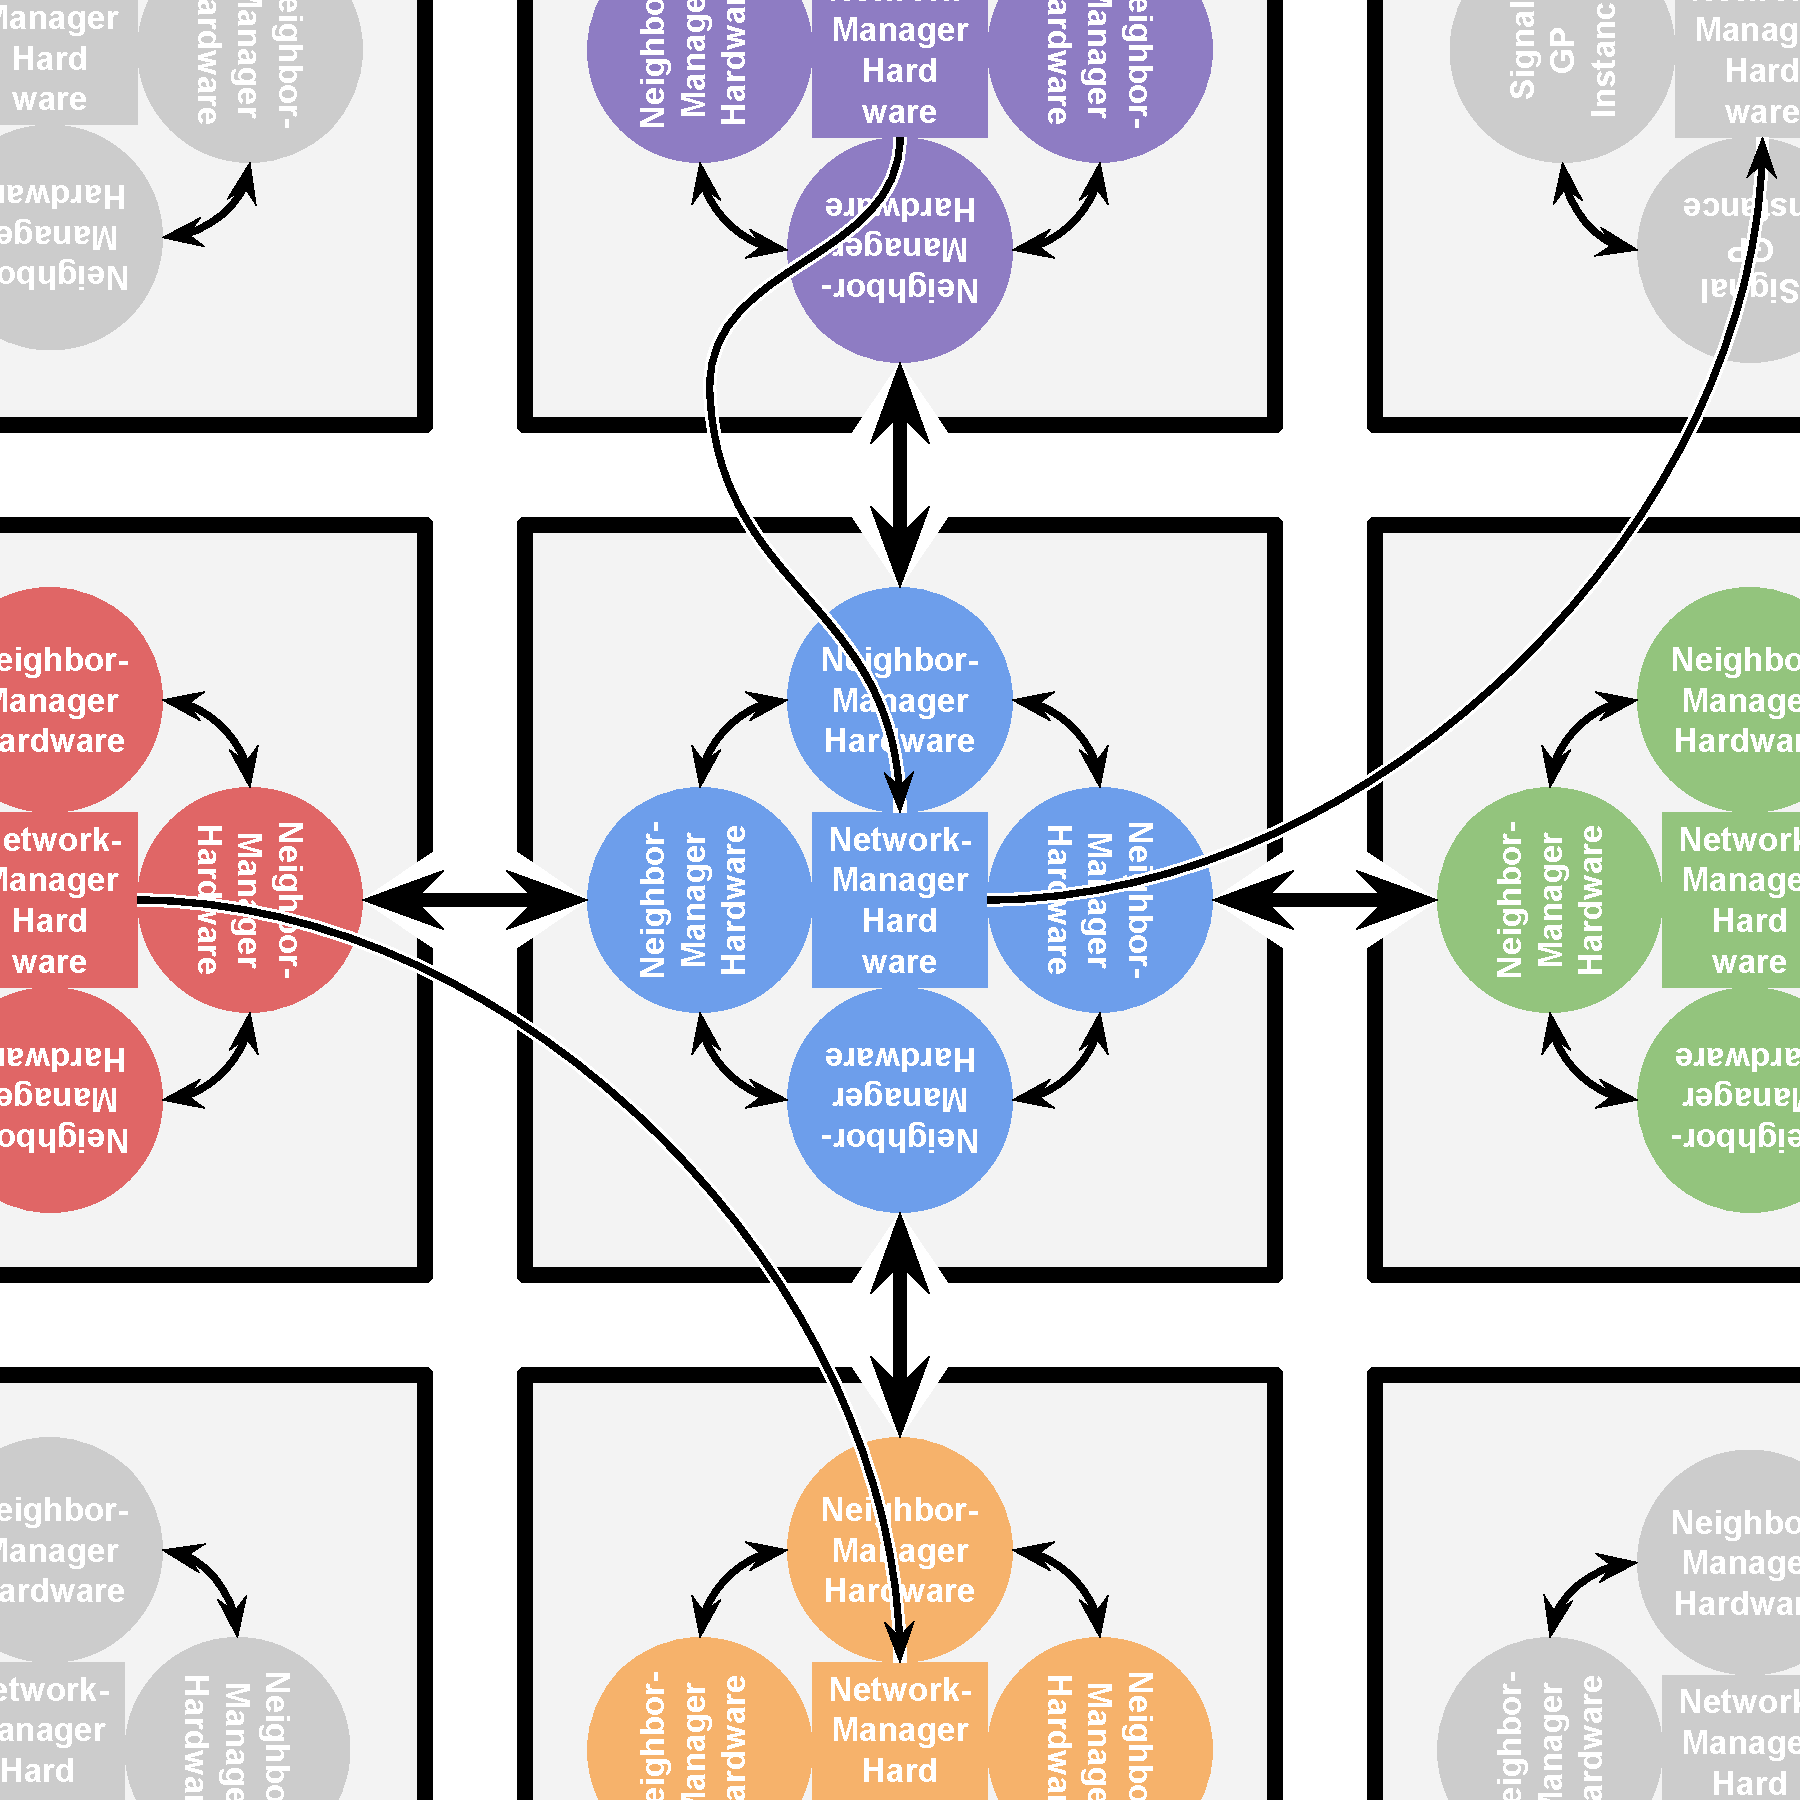
\includegraphics[width=0.7\linewidth]{img/spiker-pointer-hardware.pdf}
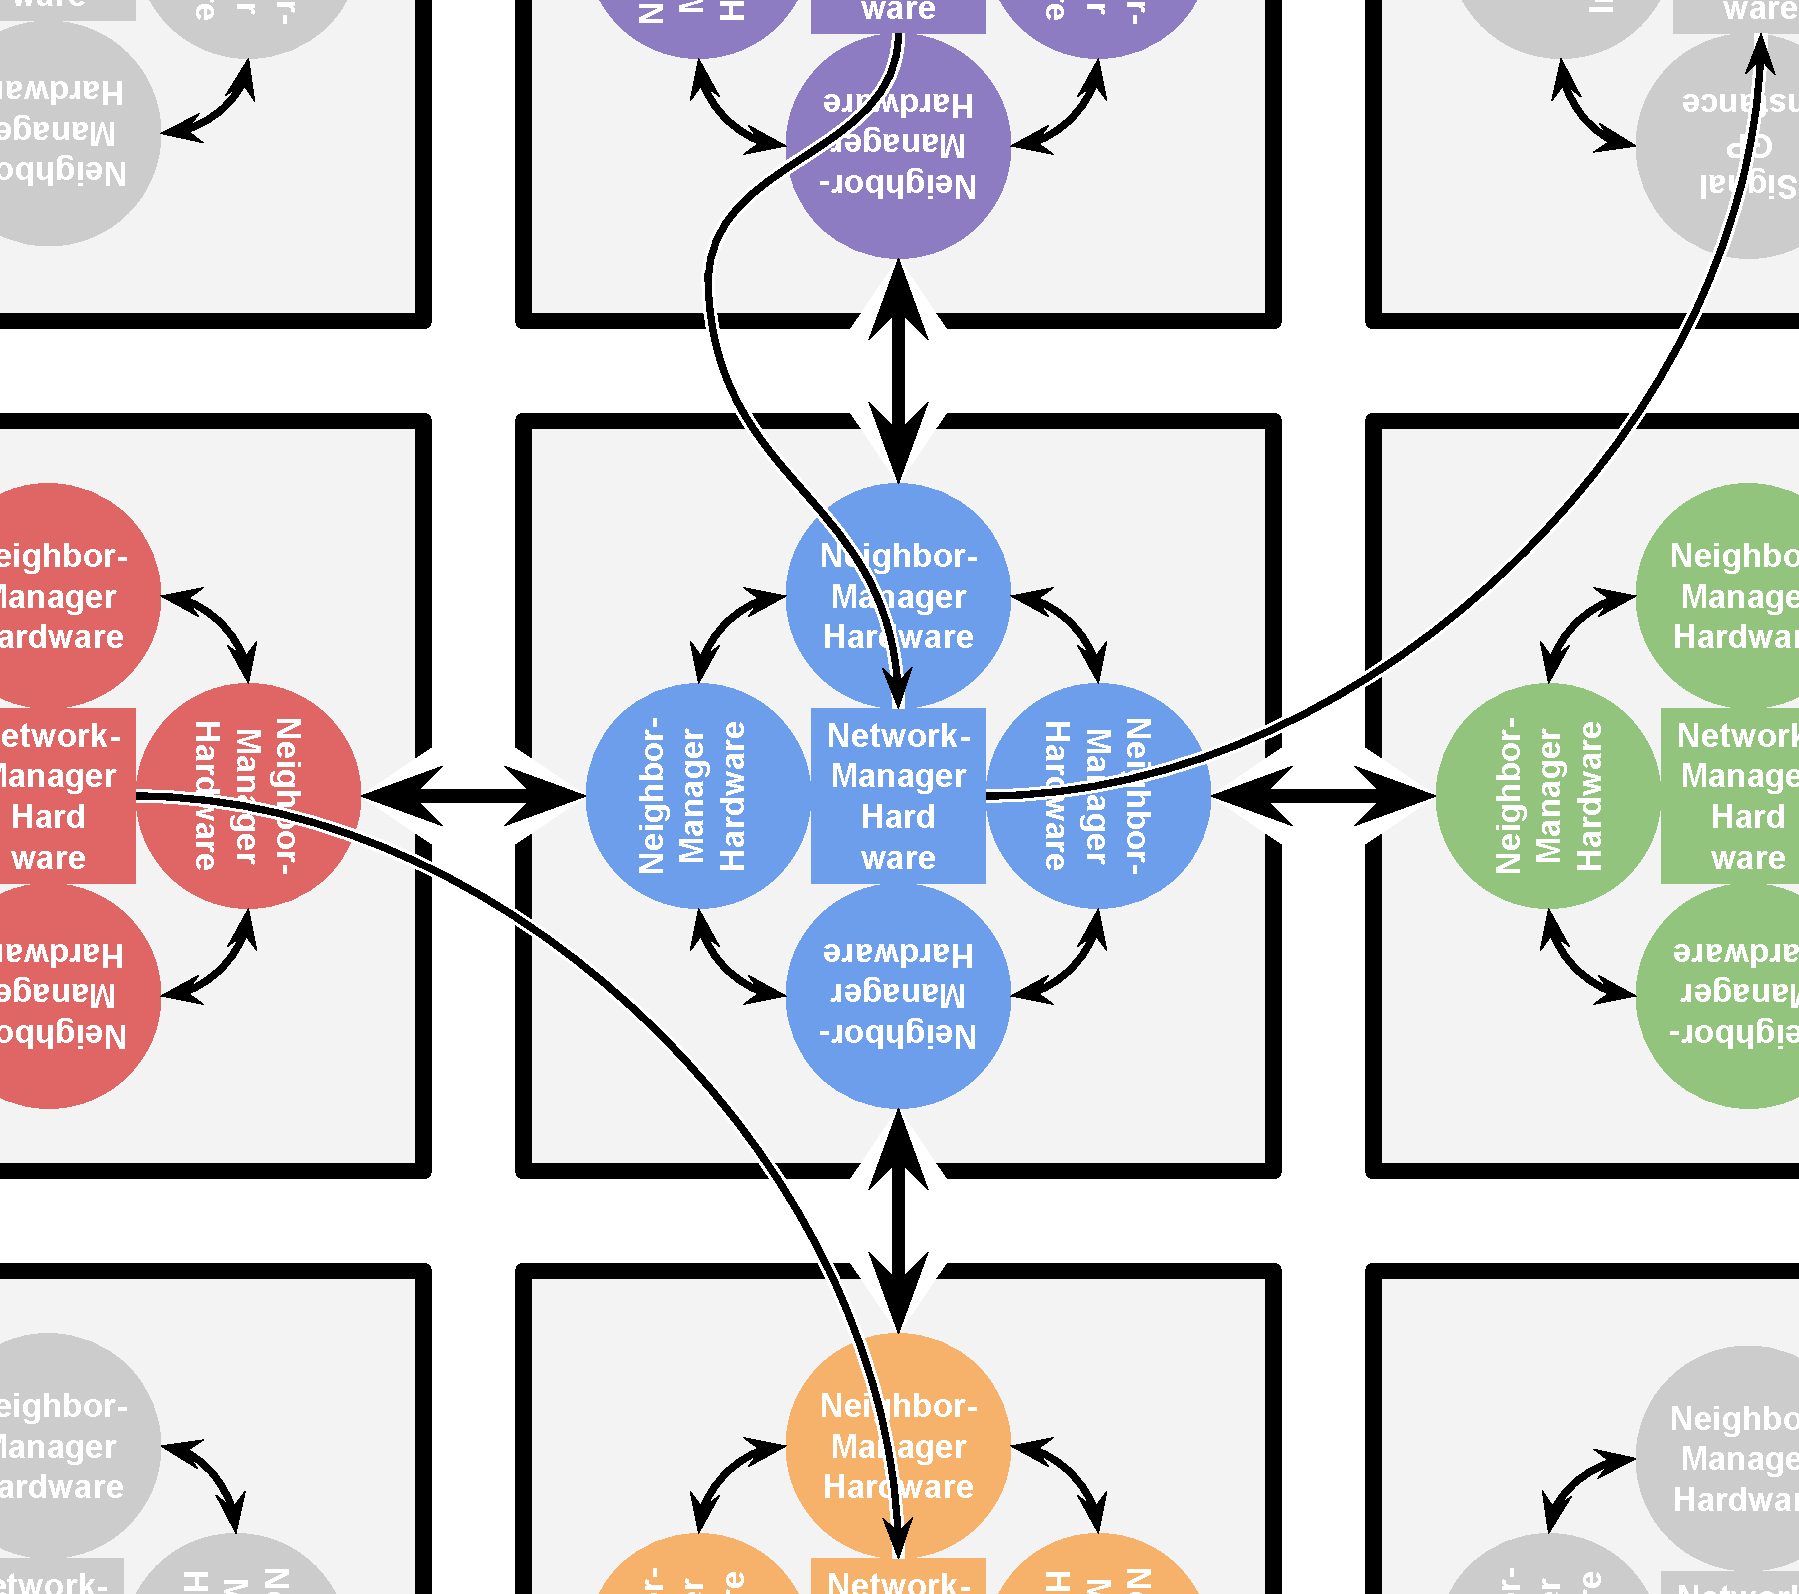
\includegraphics[width=0.8\linewidth]{img/spiker-pointer-hardware2.pdf}
\caption{
Arrangement of SignalGP hardware within DISHTINY cells (gray squares).
Neighbor-managing hardware (circles) receive stimuli and control cell behavior with respect to a particular cell neighbor.
Network-managing hardware (interior squares) receive stimuli and controll cell behavior with respect to more distant neighbors a cell has established interconnects with.
}
\label{fig:spiker_pointer_hardware}
\end{center}
\end{figure}


\begin{figure*}[!htbp]
\begin{center}
\begin{subfigure}[b]{0.33\linewidth}
  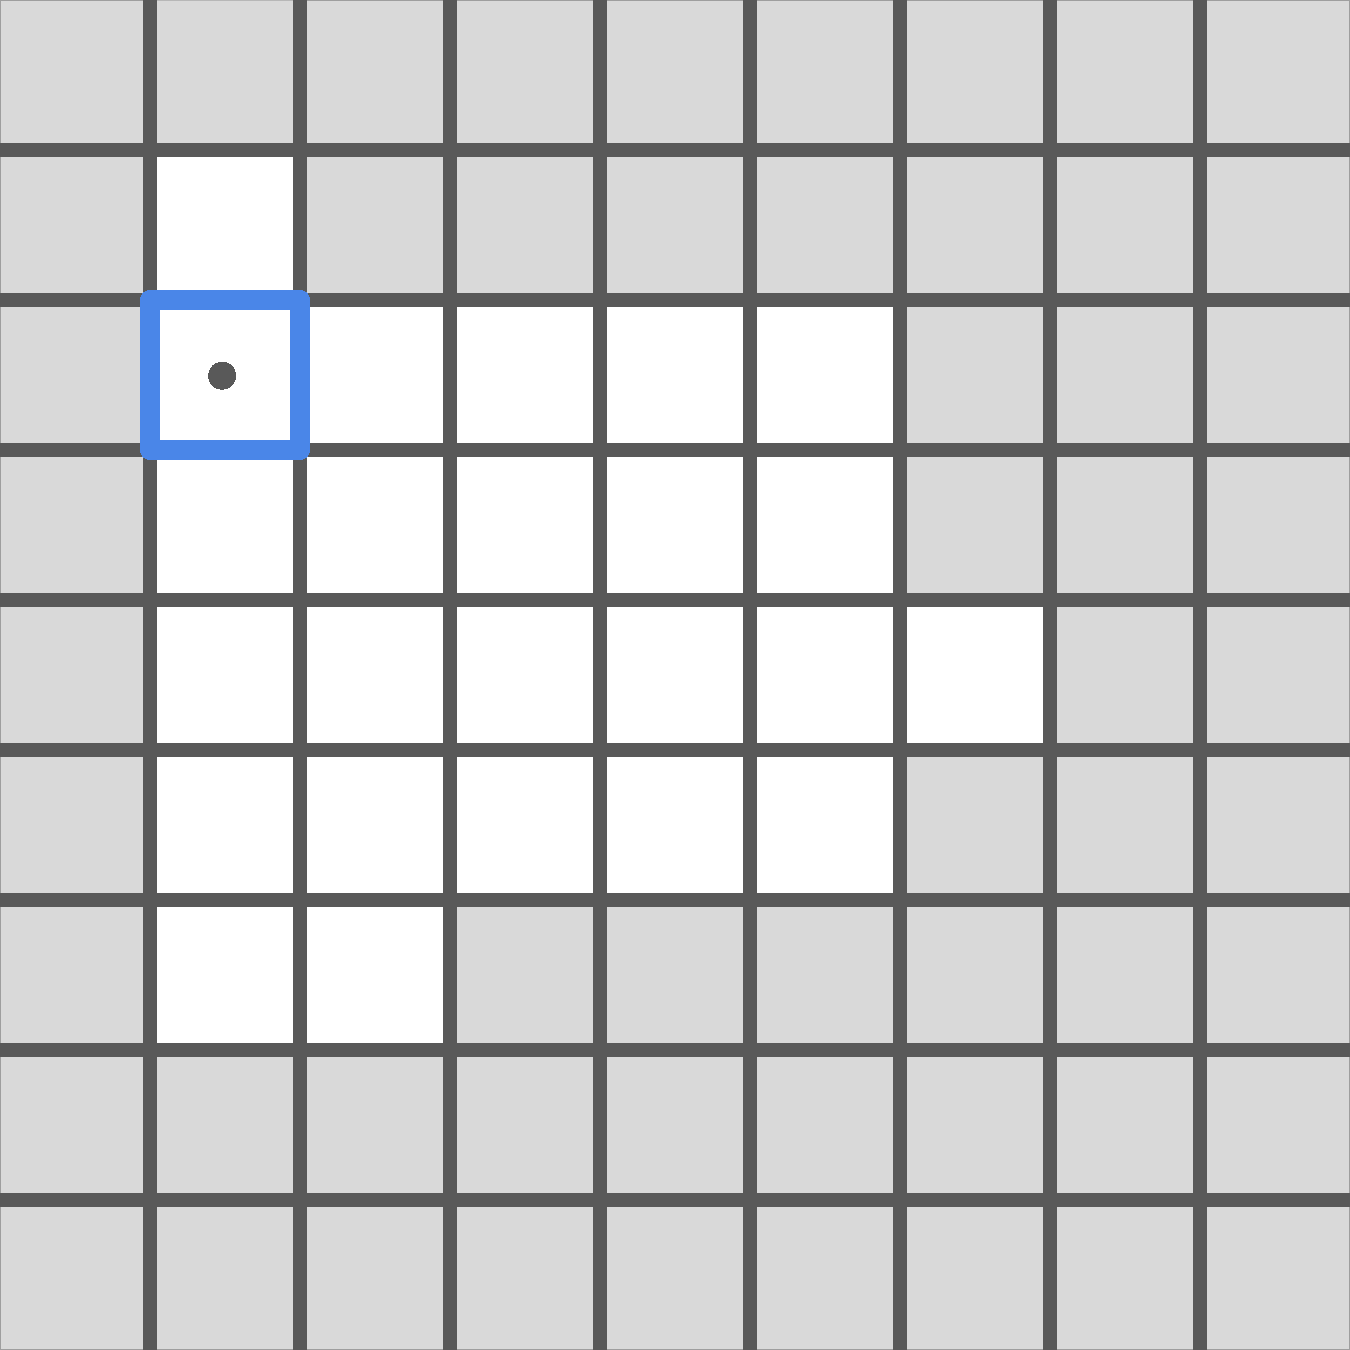
\includegraphics[width=\linewidth,trim={0 100 100 0},clip]{spiker-diagram/spiker-generate}
  \caption{TODO}
  \label{fig:TODO}
\end{subfigure}
\begin{subfigure}[b]{0.33\linewidth}
  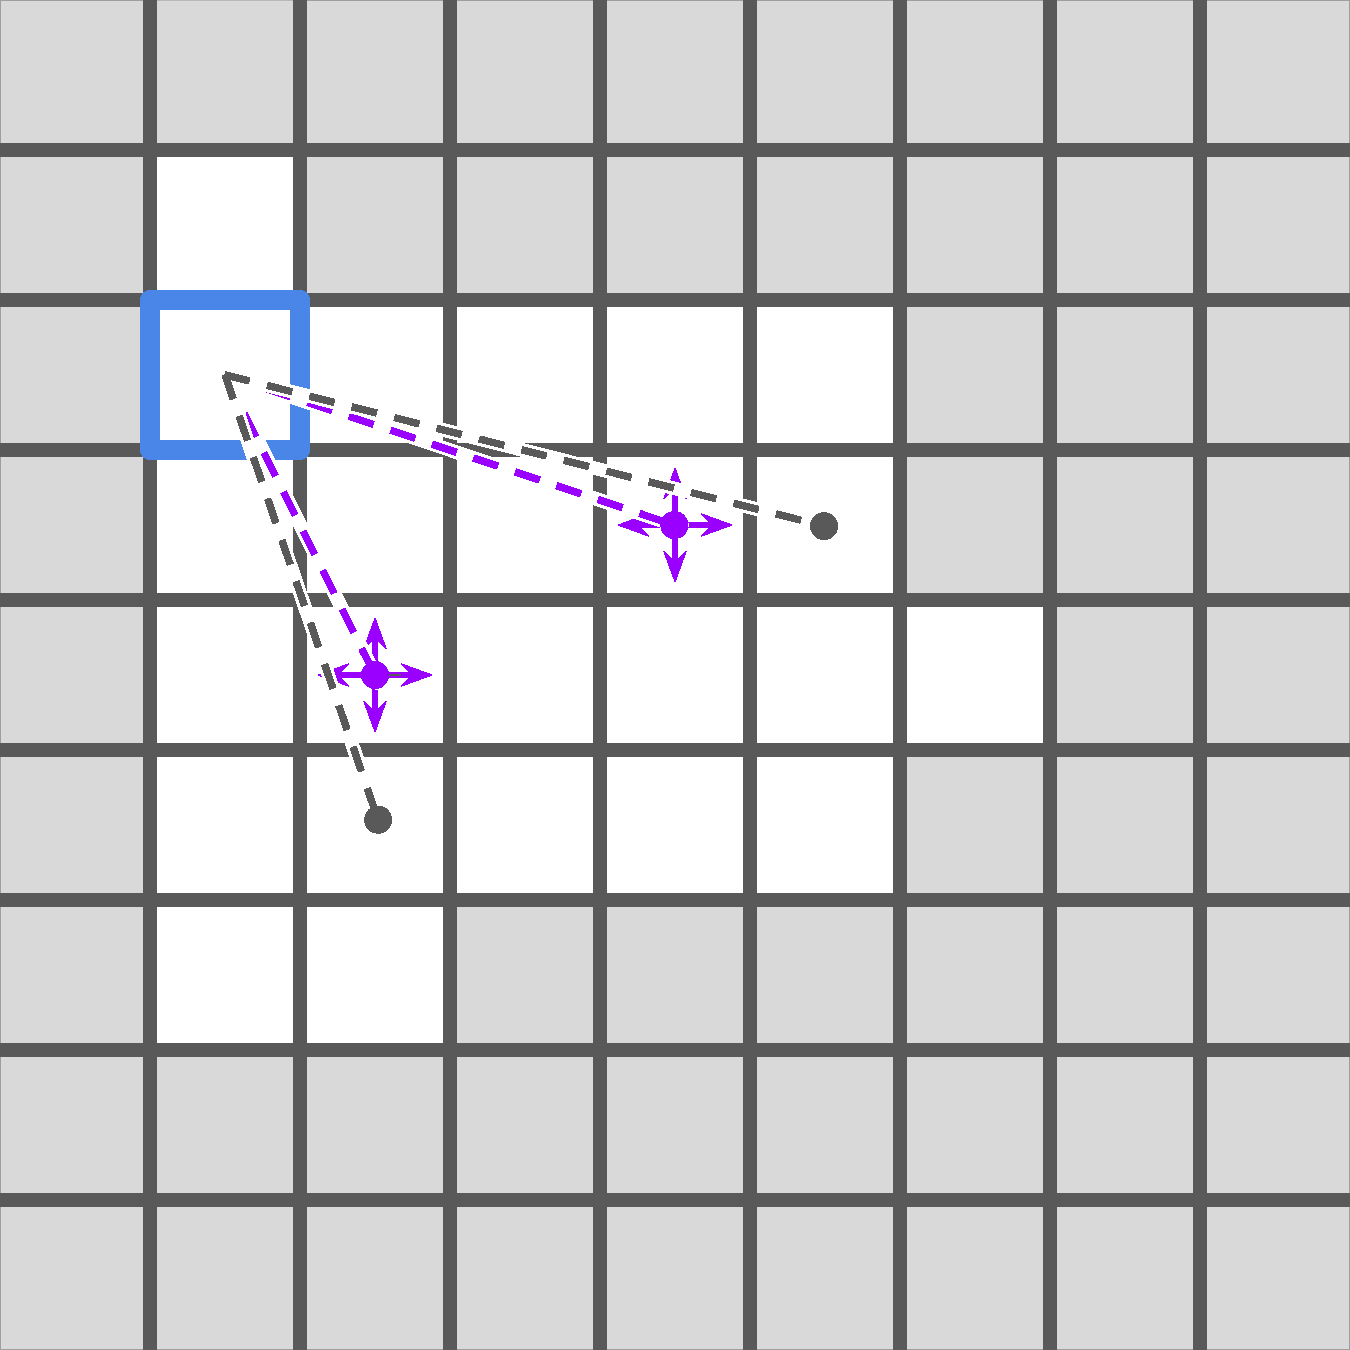
\includegraphics[width=\linewidth,trim={0 100 100 0},clip]{spiker-diagram/spiker-walk}
  \caption{TODO}
  \label{fig:TODO}
\end{subfigure}
\begin{subfigure}[b]{0.33\linewidth}
  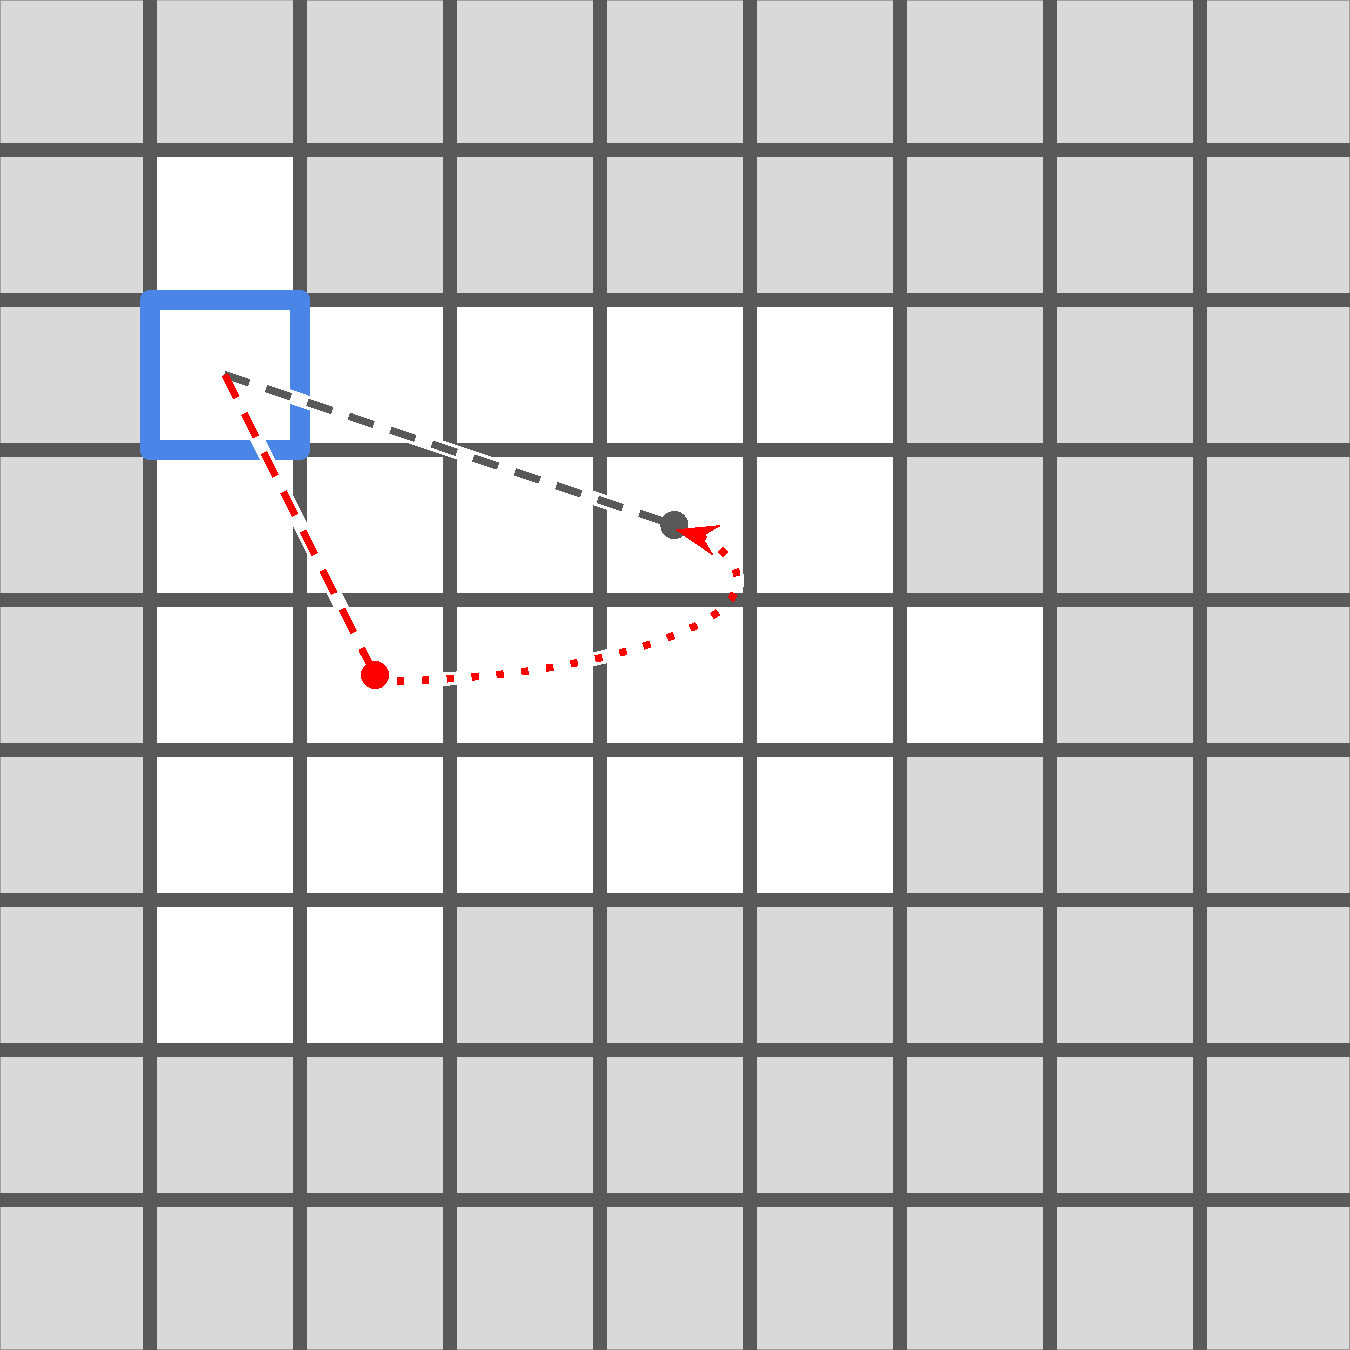
\includegraphics[width=\linewidth,trim={0 100 100 0},clip]{spiker-diagram/spiker-swap}
  \caption{TODO}
  \label{fig:TODO}
\end{subfigure}
\begin{subfigure}[b]{0.33\linewidth}
  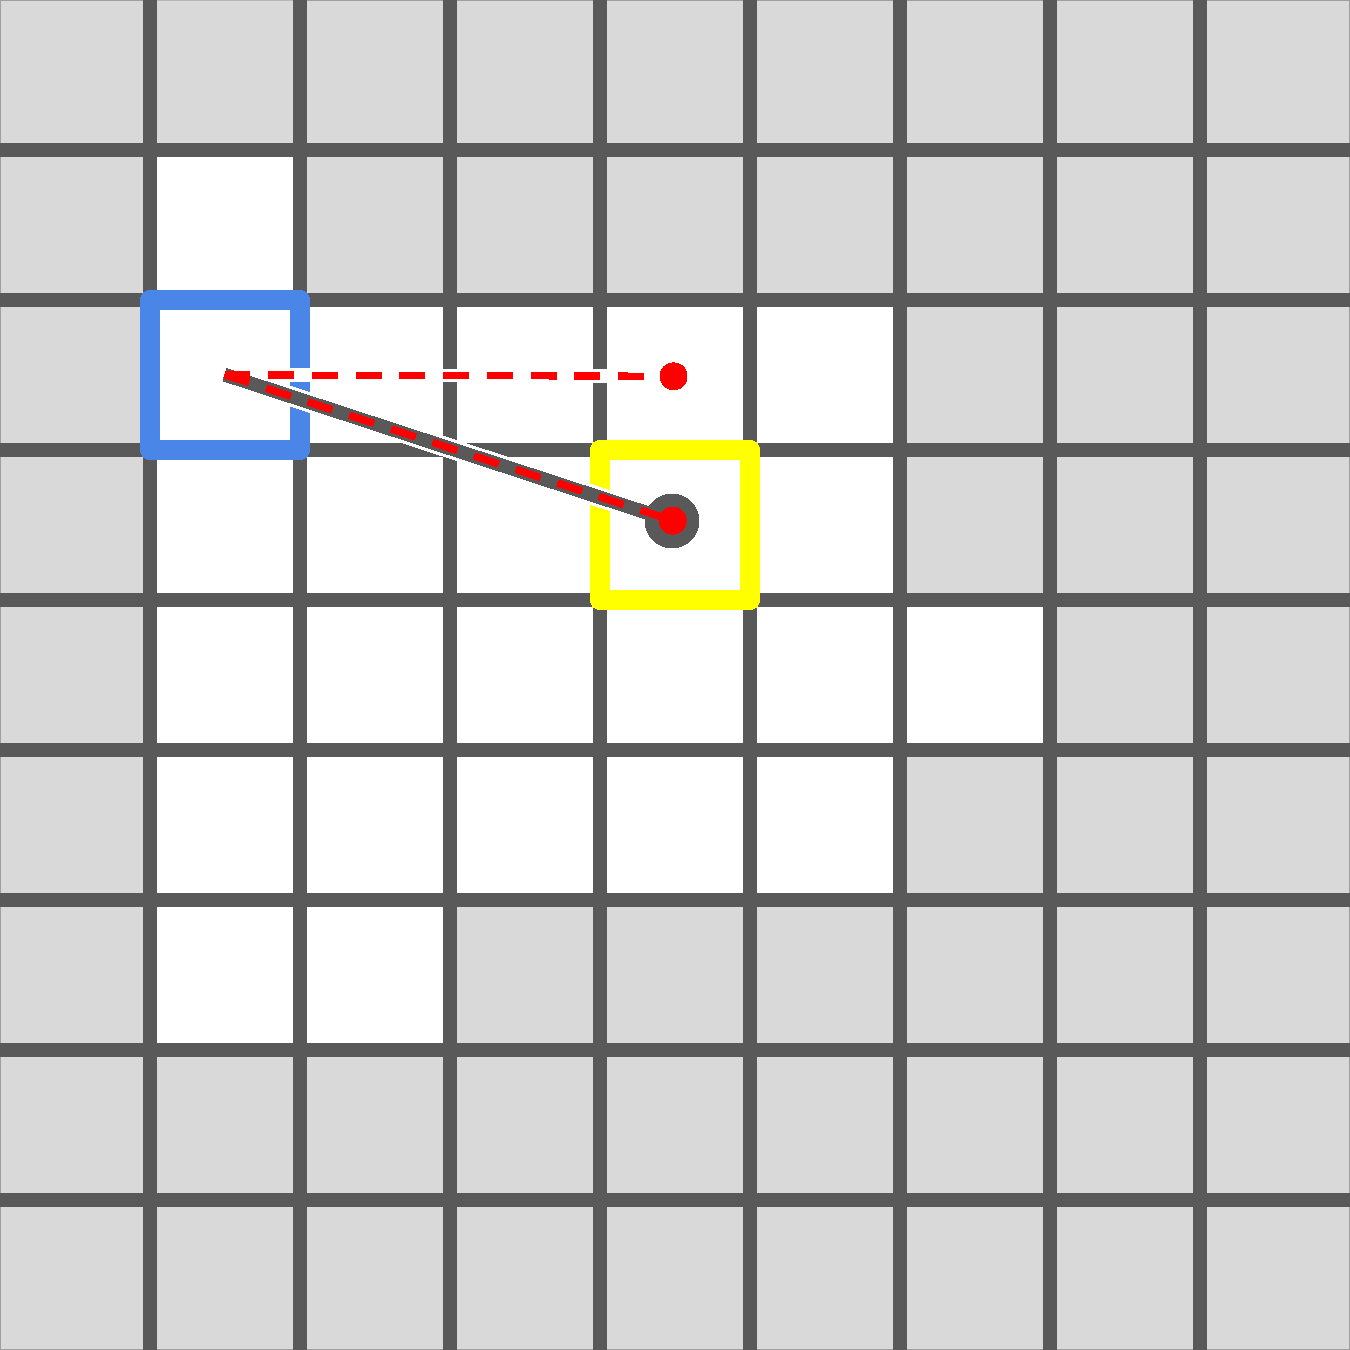
\includegraphics[width=\linewidth,trim={0 100 100 0},clip]{spiker-diagram/spiker-connect}
  \caption{TODO}
  \label{fig:TODO}
\end{subfigure}
\begin{subfigure}[b]{0.33\linewidth}
  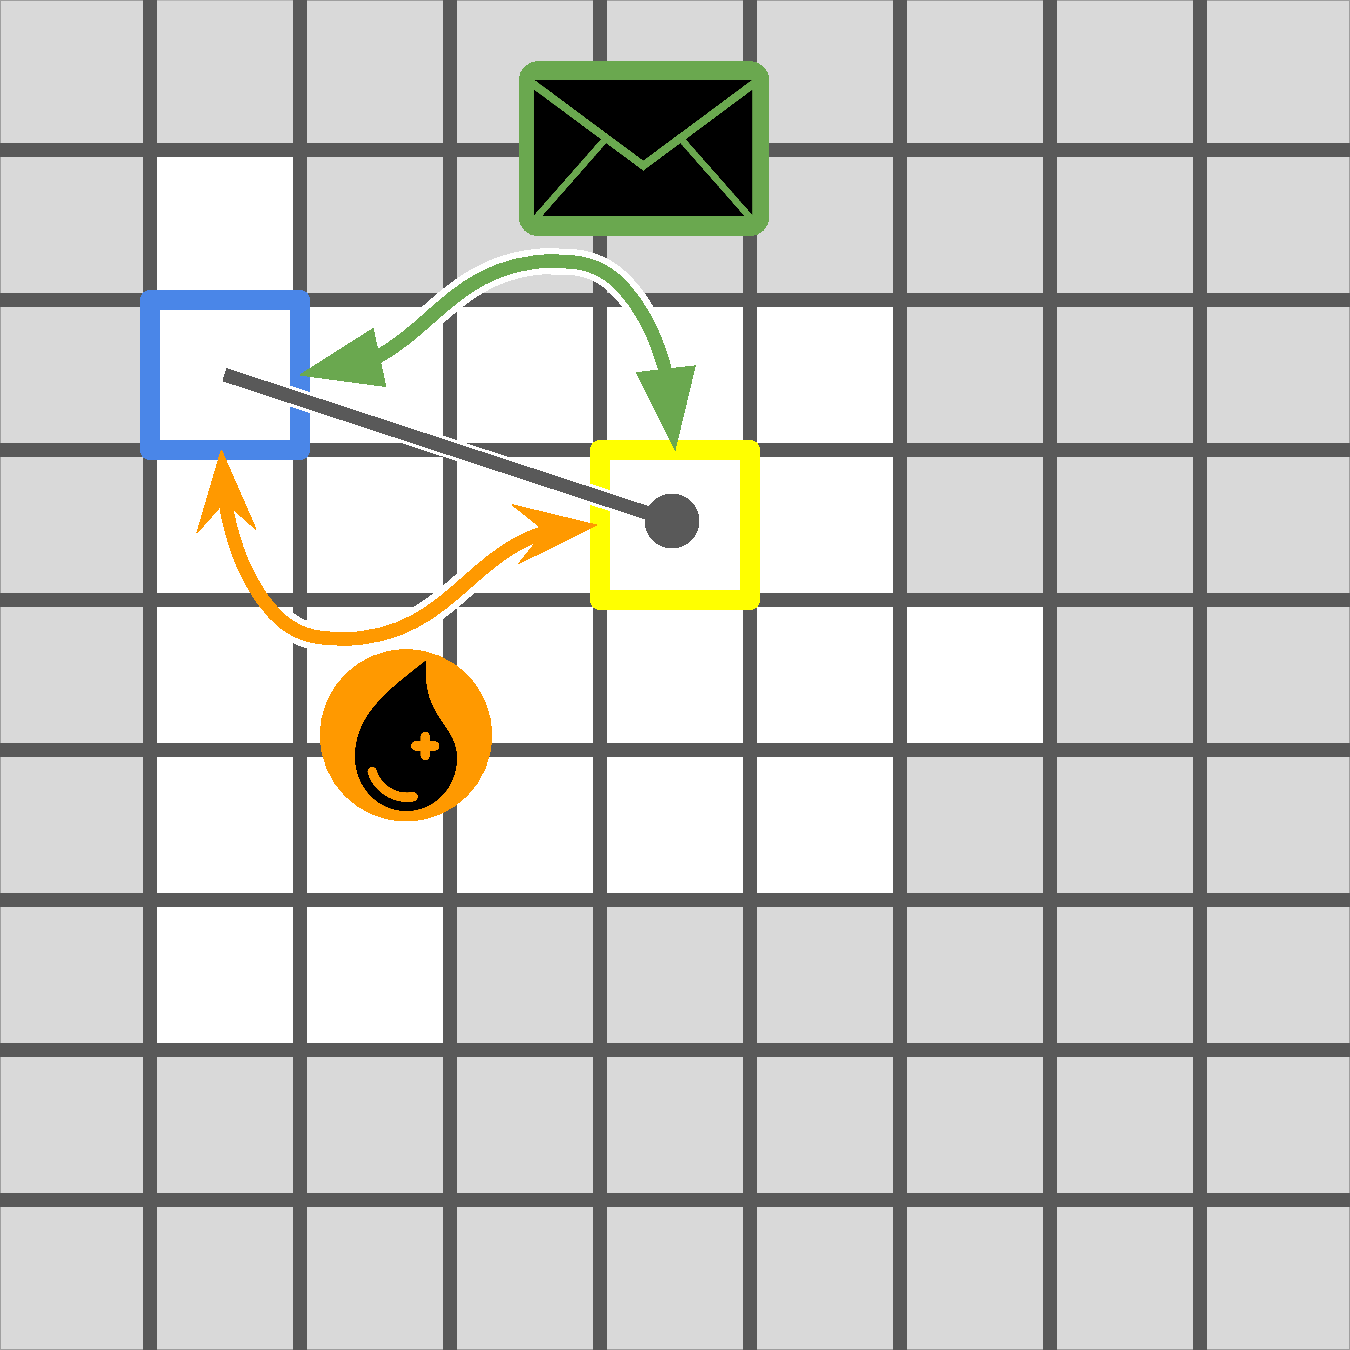
\includegraphics[width=\linewidth,trim={0 100 100 0},clip]{spiker-diagram/spiker-transmit}
  \caption{TODO}
  \label{fig:TODO}
\end{subfigure}
\begin{subfigure}[b]{0.33\linewidth}
  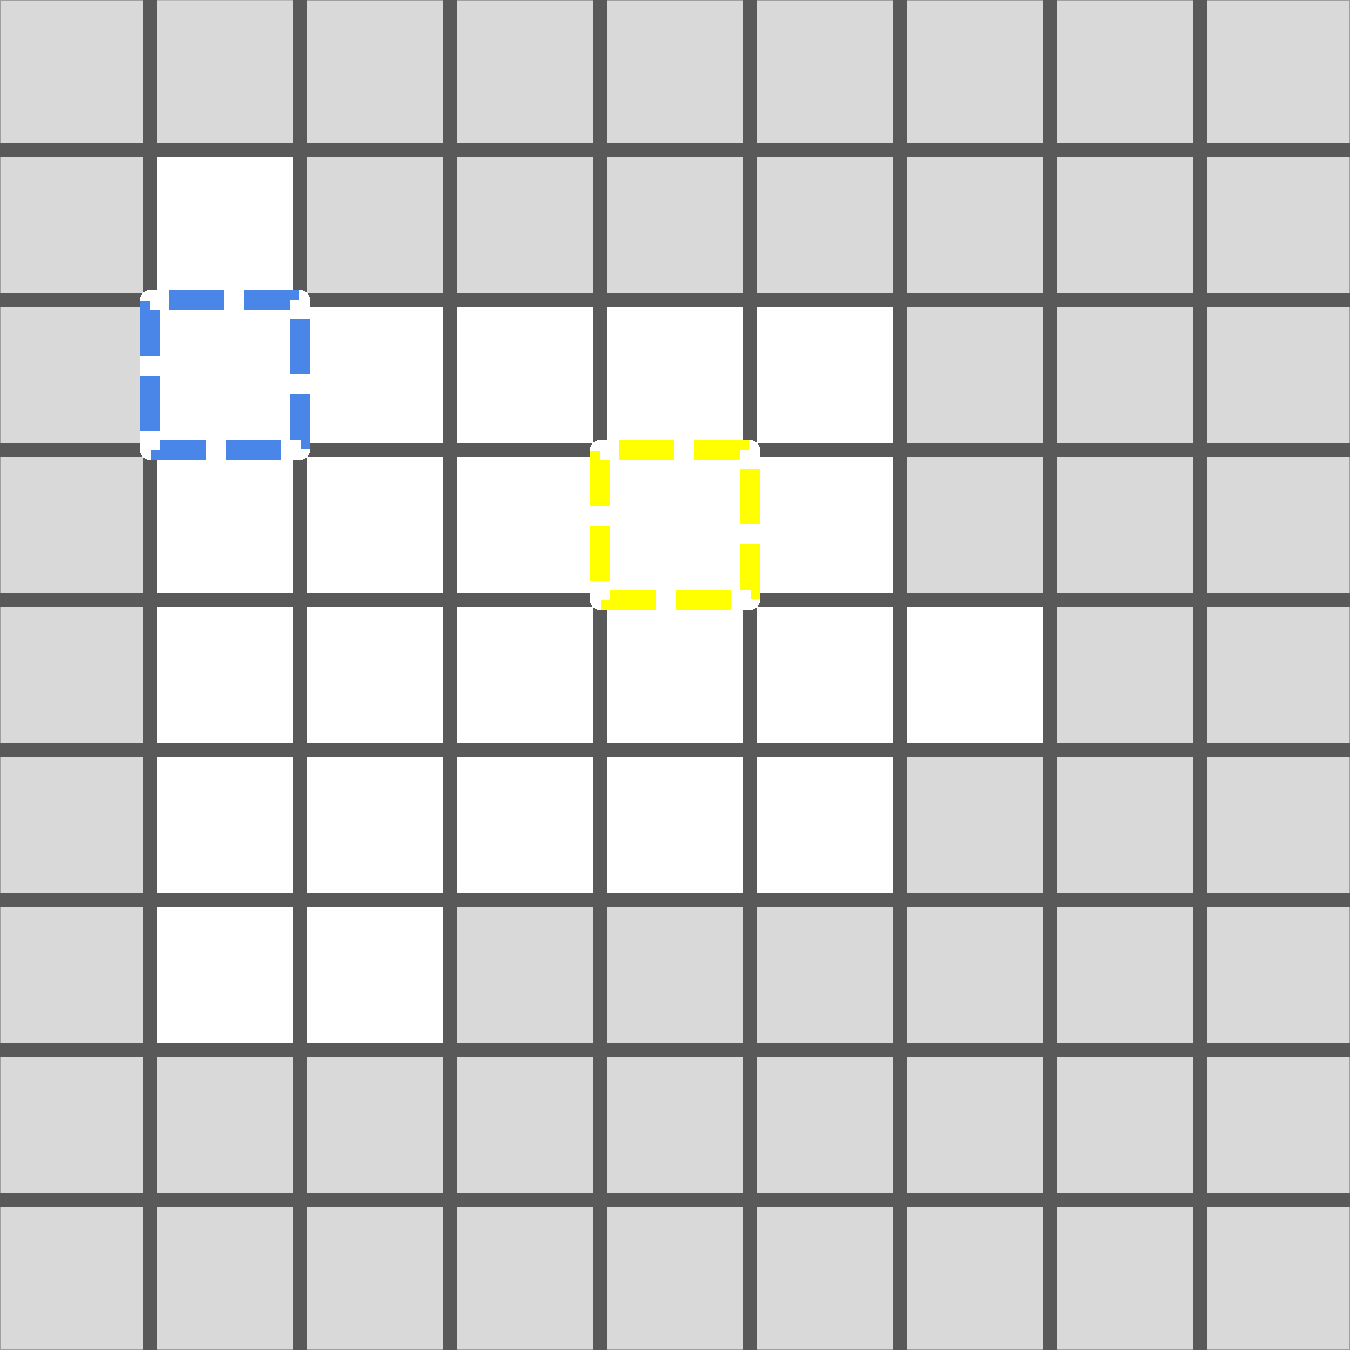
\includegraphics[width=\linewidth,trim={0 100 100 0},clip]{spiker-diagram/spiker-remove}
  \caption{TODO}
  \label{fig:TODO}
\end{subfigure}
\caption{
TODO
}
\label{fig:spiker_diagram}
\end{center}
\end{figure*}


\subsection{Evolutionary Screens}

We running 64 replicate batches in 4-hour steps.
Each batch consisted of four isolated subpopulations, which were completely intermixed in between four-hour steps.

We screened across four-hour checkpoints of replicate batches to see if messages or resource were being sent over interconnects.
We sampled from these populations, performing screens for knockouts of interconnect messaging or resource sharing.
We found several evolved genotypes that used interconnects adaptively.
We then further screened to ensure that the intra-cellular nature of the interconnects were vital by testing to see whether connecting interconnects to the originating cells themselves after the developmental process affected fitness.

We continued this process until we found a strain where interconnects were used for resource sharing and a strain where interconnects were used for cell-cell messaging.

We did not find a strain where resource sharing was used outside of the context of interconnect resource sharing in the main set of set or runs.
So we performed a secondary set of runs with several adjustments and different seeds, including:
\begin{enumerate}
  \item increasing the default outgoing connection cap and
  \item making cells default-accept instead of default-reject intracellular messages from same-channel cells.
\end{enumerate}

We repeated the screening process on the secondary process, finding a strain where interconnects were used for adaptive cell-cell messaging outside the context of resource sharing over the interconnect.

\subsection{Implementation}

We implemented our experimental system using the Empirical library for scientific software development in C++, available at \url{https://github.com/devosoft/Empirical} \citep{TODOcite}.
We used OpenMP to parallelize our main evolutionary replicates, distributing work over two threads.
The code used to perform and analyze our experiments, our figures, data from our experiments, and a live in-browser demo of our system is available via the Open Science Framework at \url{https://osf.io/TODO/}.


\section{Results and Discussion}

\subsection{Scaling Relationship of Node-to-Node Transfers per Connection of Small World Graph on Toroidal Grid} \label{sec:scaling_toroidal}

We will consider a set of computational nodes $N$.
These nodes are arranged toroidally so that, in each dimension, each ...
Physical interconnects

Let $d$ represent the typical number of physical interconnects traversed on a shortest path between a pair of arbitrary nodes $a, b \in N$.
This is conceptually equivalent to Manhattan distance.
In the case of a one-dimensional ring topology,
\begin{align*}
d(a,b) \propto |N|.
\end{align*}

In the case of a higher-dimensional toroidal grid topology, like a two-dimensional grid or a three-dimensional mesh, by taxicab properties the number of physical interconnects required to be traversed between two nodes in different dimensions are completely independent.
For a $n$-dimensional grid, grid width in each dimensions scales proportionally to the $n$-th root of of grid size.
From this point forward, we will assume a three-dimensional mesh, so for a pair of arbitrary nodes $a,b \in N$,
\begin{align*}
d(a, b) \propto |N|^{\frac{1}{3}}
\end{align*}

We will superimpose a small world directed graph $G$ over the network.
Each node in this graph corresponds bijectively to a member of $N$.
Edges in this graph represent a close-coordination relationship, where the source node frequently dispatches messages to the destination node.
These edges do not correspond to physical interconnects.

By the definition of a small-world network, the typical graph-distance $\hat{d}$ (the number of graph edges traversed on a shortest-path route) between a pair of arbitrary nodes $\hat{a},\hat{b} \in G$ scales proportionally with the logarithm of the network size,
\begin{align*}
\hat{d}(\hat{a},\hat{b}) \propto \log(|G|).
\end{align*}

By definition, there cannot exist
(a shorter physical interconnect distance)

So, for a shortest-path $r(a,b)$,
\begin{align*}
\sum_{e \in r(a,b)} d(e) \leq d(a,b).
\end{align*}

Hence,
\begin{align*}
\sum_{e \in r(a,b)} d(e) \in O(|N|^{\frac{1}{3}})
\end{align*}

In aggregate,
\begin{align*}
\log(|N|) \times d(e) \in O(|N|^{\frac{1}{3}})
\end{align*}

So,
\begin{align*}
d(e) \in O(|N|^{\frac{1}{3}} / \log(|N|))
\end{align*}


\begin{figure}[!htbp]
\begin{center}
\begin{subfigure}[b]{0.49\columnwidth}
  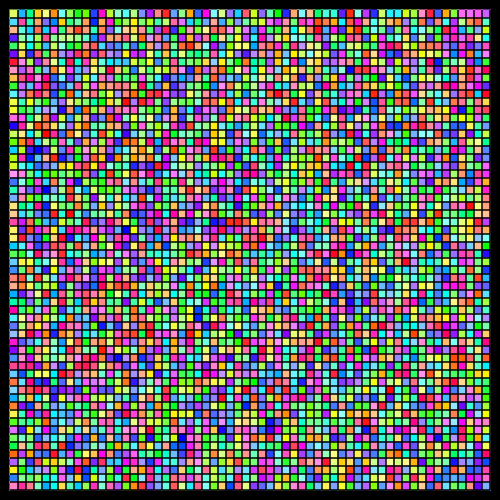
\includegraphics[width=\columnwidth]{source_hash=de48c04-dirty_emp_hash=1c7cb544-clean_title=channel_viz+treat=resource-wave__channelsense-yes__nlev-two+seed=1+update=0}
  \caption{Update 0; gen. 0}
  \label{fig:TODO}
\end{subfigure}
\begin{subfigure}[b]{0.49\columnwidth}
  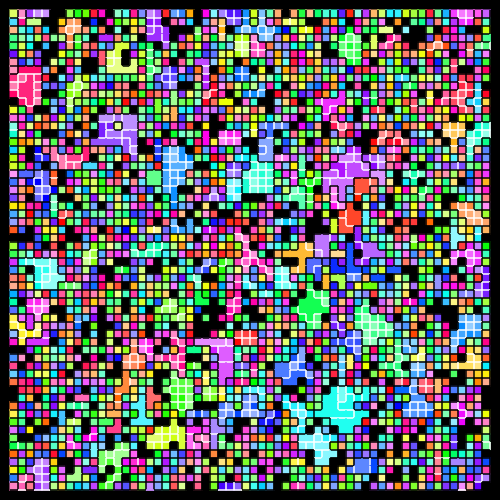
\includegraphics[width=\columnwidth]{source_hash=de48c04-dirty_emp_hash=1c7cb544-clean_title=channel_viz+treat=resource-wave__channelsense-yes__nlev-two+seed=1+update=2500}
  \caption{Update 2.5k; gen. TODO}
  \label{fig:TODO}
\end{subfigure}
\begin{subfigure}[b]{0.49\columnwidth}
  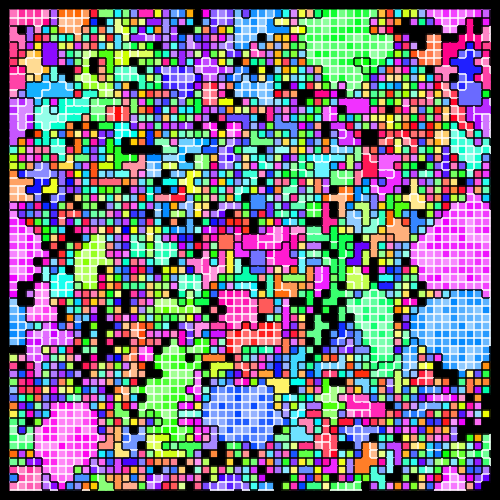
\includegraphics[width=\columnwidth]{source_hash=de48c04-dirty_emp_hash=1c7cb544-clean_title=channel_viz+treat=resource-wave__channelsense-yes__nlev-two+seed=1+update=5000}
  \caption{Update 5k; gen. TODO}
  \label{fig:TODO}
\end{subfigure}
\begin{subfigure}[b]{0.49\columnwidth}
  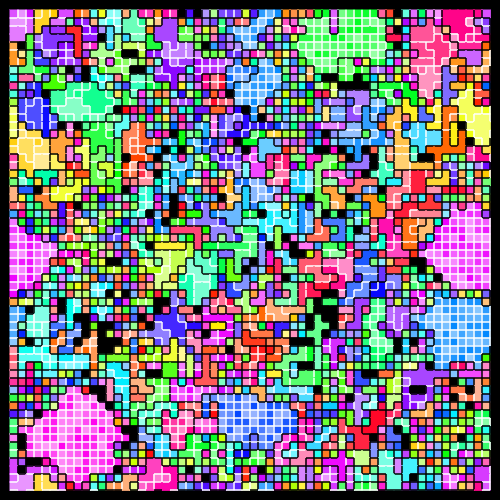
\includegraphics[width=\columnwidth]{source_hash=de48c04-dirty_emp_hash=1c7cb544-clean_title=channel_viz+treat=resource-wave__channelsense-yes__nlev-two+seed=1+update=7500}
  \caption{Update 7.5k; gen. TODO}
  \label{fig:TODO}
\end{subfigure}
\begin{subfigure}[b]{0.49\columnwidth}
  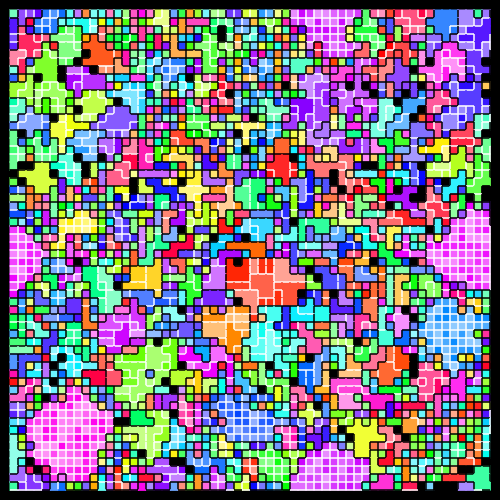
\includegraphics[width=\columnwidth]{source_hash=de48c04-dirty_emp_hash=1c7cb544-clean_title=channel_viz+treat=resource-wave__channelsense-yes__nlev-two+seed=1+update=10000}
  \caption{Update 10k; gen. TODO}
  \label{fig:TODO}
\end{subfigure}
\begin{subfigure}[b]{0.49\columnwidth}
  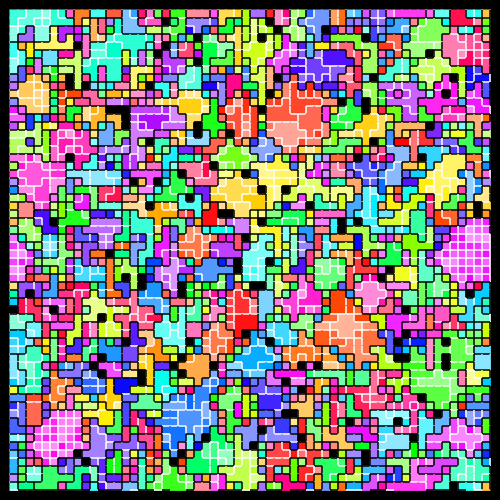
\includegraphics[width=\columnwidth]{source_hash=de48c04-dirty_emp_hash=1c7cb544-clean_title=channel_viz+treat=resource-wave__channelsense-yes__nlev-two+seed=1+update=20000}
  \caption{Update 20k; gen. TODO}
  \label{fig:TODO}
\end{subfigure}
\begin{subfigure}[b]{0.49\columnwidth}
  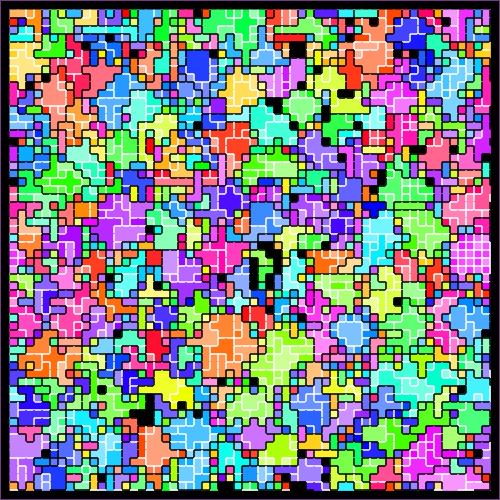
\includegraphics[width=\columnwidth]{source_hash=de48c04-dirty_emp_hash=1c7cb544-clean_title=channel_viz+treat=resource-wave__channelsense-yes__nlev-two+seed=1+update=30000}
  \caption{Update 30k; gen. TODO}
  \label{fig:TODO}
\end{subfigure}
\begin{subfigure}[b]{0.49\columnwidth}
  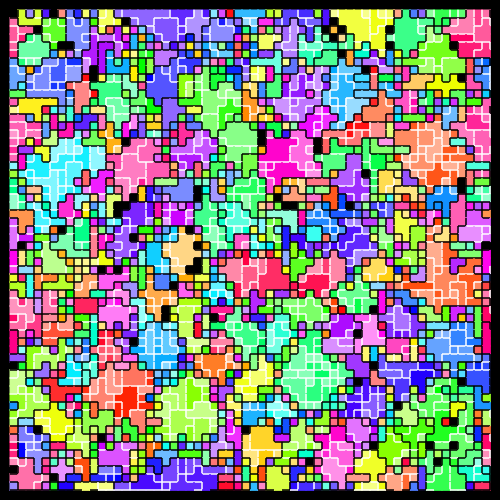
\includegraphics[width=\columnwidth]{source_hash=de48c04-dirty_emp_hash=1c7cb544-clean_title=channel_viz+treat=resource-wave__channelsense-yes__nlev-two+seed=1+update=50000}
  \caption{Update 50k; gen. TODO}
  \label{fig:TODO}
\end{subfigure}
\caption{
Progression of of same-channel level-zero and level-one signaling networks states in an evolutionary run.
In the "Channel Viewer", low-level groups are coded by color saturation (divided by white lines) and high-level groups are coded by color hue (divided by black lines).
Black grid tiles represent empty channel ID.
}
\label{fig:grid_progression}
\end{center}
\end{figure}


\subsection{TODO}

Figure \ref{fig:grid_progression}

standard versus blind+even ($p < 0.05$; bootstrap test)
small wave versus blind+even ($p < 0.01$; bootstrap test)


\section{Conclusion}

Ackley's concept of indefinite scalability lays out an ambitious vision for the computational substrate of future open-ended evolution models.
This vision has inspired researchers to incorporate thinking about underlying computational substrates into open-ended evolution theory and consider how (or whether) available computational resources meaningfully constrain existing open-ended evolution models.
Although computational substrates for open-ended evolution limited purely by physical (or economic) concerns have yet to be realized, indefinite scalability has already had concrete, and fruitful, impact on thinking around open-ended evolution.

Although prevalent contemporary computational hardware (and the developer-facing software infrastructure that supports its use) lacks essential features necessary to achieve true indefinite scalability such as fault tolerance and purely relative addressing, many cores designed to support low-latency interconnects.
These high-performance computing resources are increasingly accessible.
Concern over indefinite scalability should not disuade the design and implemenation of open-ended evolution models that accomodate for the limitations of existing hardware and softare infrastructure to make effective use of it.
We highlight how log-time hardware interconnects might be exploited in practically scalable, but other model design or implementation tradeoffs may be relevant too (e.g., model dynamics or performance gains that rely on absolute instead of purely relative addressing).

Realizing open-ended evolution models with truly vast computational substrates will require intermediate steps.
Efforts to pursue practical scalability that wrings out contemporary, commercially-available hardware and software infrastructure, will accelerate progress toward realizing truly indefinitely scalable systems.
It seems conceivable that, coupled with innovative model design informed by open-ended evolution theory and effective model implementation in codei, contemporary hardware systems and software infrastructure harbor the potential to realize paradigm-shifting advances in open-ended evolution.
As was the case with deep learning, the tipping point of scale for model systems to exhibit qualatitively different behavior may be closer than we assume, perhaps only two or three orders of magnitude.

We highlighted how dynamic interactions within and between evolutionary individuals are crucial to open-ended evolution.
Open-ended evolution models designed to scale computationally should realize these dynamic interactions within a framework that can be efficiently and readily mapped onto parallel computational implementation.
Software tools that enable artificial life researchers to rapidly (and reusably) develop artificial life models have yielded substantial benefit to the field \citep{bohm2017mabe, charles_ofria_2019_2575607}.
Software tools or frameworks for parallel and distributed artificial life models that are versatile enough to support diverse use cases might help make practical scalability more practical.
In particular, tools to collect data on distributed evolving systems (especially systematics tracking) seem likely to benefit the community.

Here, we presented an extension of the DISHTINY framework as an example of an artificial life system that might hypothetically take advantage of log-time hardware interconnects.
We employed a very modest prototype parallel implementation that used shared-memory parallelism to distribute evolving --- and interacting --- populations of cells over two threads.
We provided a faculty for cells to establish long-distance interconnects over the computational mesh, which in future implementations could rely on hardware-level log-time interconnects.
Two case studies characterized strains that evolved to adaptively employ these interconnects.
In the first, messaging and resource sharing over interconnects appeared to facilitate resource recruitment to multicell peripheries.
In the second, interconnect messaging played an adaptive role in selectively moderating somatic reproduction.

Incorporating simulation-level objects or physics in open-ended evolution models that explicitly correspond to hardware interconnects represents just one possible approach to exploiting them.
Automatic detection of emergent long-distance interactions across a computational mesh and dynamically re-routing signaling traffic to use hierarchical interconnects might also be possible.
Open-ended evolution models could also be entirely designed around hierarchical interconnects instead of a space-filling computational mesh.

At the core, from both the practical and indefinite standpoints, efforts to scale computational models of open-ended evolution, seek to realize the evolutionary generation of continually novel and increasingly complex artifacts.
As we scale DISHTINY, we are interested in assembling metrics to quantify different aspects of complexity in the system such as organization \citep{goldsby2012task}, structure, and function \citep{goldsby2014evolutionary}.
We hope that parallel and distributed open-ended model systems will prove fruitful tools to investigate questions about how biological complexity relates to fitness, genetic drift over elapsed evolutionary time, mutational load, genetic recombination (sex and horizontal gene transfer), ecology, historical contingency, and key innovations.



\section{Acknowledgements}

Thanks to members of the DEVOLAB, in particular TODO for help with TODO.
This research was supported in part by NSF grants DEB-1655715 and DBI-0939454, and by Michigan State University through the computational resources provided by the Institute for Cyber-Enabled Research.
This material is based upon work supported by the National Science Foundation Graduate Research Fellowship under Grant No. DGE-1424871.
Any opinions, findings, and conclusions or recommendations expressed in this material are those of the author(s) and do not necessarily reflect the views of the National Science Foundation.


\footnotesize
\bibliographystyle{apalike}
\bibliography{bibl} % replace by the name of your .bib file

\clearpage
\newpage

\appendix

\subsection{Standard SignalGP Instruction Library}

To counteract crowding of the mutational landscape by the volume of custom instructions provided, a second identical copy of each standard SignalGP instruction was included in the library.
These instructions were included in both the neighbor hardware and network hardware instruction libraries.

\begin{itemize}
\item \textbf{Increment}
Increment value in a designated register.
\item \textbf{Decrement}
Decrement value in a designated register.
\item \textbf{Not}
Logically toggle value in a designated register.
\item \textbf{Add}
Add values from two designated registers into a third designated register.
\item \textbf{Subtract}
Subtract values from two designated registers into a third designated register.
\item \textbf{Subtract}
Subtract values from two designated registers into a third designated register.
\item \textbf{Multiply}
Multiply values from two designated registers into a third designated register.
\item \textbf{Divide}
Divide values from two designated registers into a third designated register.
\item \textbf{Modulus}
Calculate the modulus from two designated registers and place result into a third designated register.
\item \textbf{Test Equal}
Compare values in two designated registers and place equality result into a third designated register.
\item \textbf{Test Non-equality}
Compare values in two designated registers and place opposite equality result into a third designated register.
\item \textbf{Test Less}
Compare values in two designated registers and place less-than result into a third designated register.
\item \textbf{If}
If a designated register is non-zero, proceed.
Otherwise, skip block.
\item \textbf{While}
While a designated register is non-zero, loop over a program block.
Otherwise, skip block.
\item \textbf{Countdown}
While a designated register is non-zero, loop over a program block and decrement the value in the designated register.
Otherwise, skip block.
\item \textbf{Close}
If a preceding program block is, close it.
\item \textbf{Break}
Break to the end of the current program block.
\item \textbf{Call}
Call the SignalGP program module that best matches instruction's affinity.
\item \textbf{Return}
If possible, return from the current function.
\item \textbf{Set Memory}
% also covers terminal
Set a designated register's value to genetically-determined value.
\item \textbf{Copy Memory}
Copy the value of a designated register to a second designated register.
\item \textbf{Swap Memory}
Swap the values of two designated registers.
\item \textbf{Input}
Copy a designated element of input memory into a designated register.
\item \textbf{Output}
Copy to a designated element of output memory from a designated register.
\item \textbf{Commit}
Copy a designated register into a designated element of global memory.
\item \textbf{Pull}
Copy a designated element of global memory into a designated register.
\item \textbf{Fork}
Fork a new thread with the SignalGP program module that best matches the instruction's affinity.
\item \textbf{Terminate}
Terminate the current thread.
\item \textbf{Nop}
No operation.
\item \textbf{RNG Draw}
Draw a random value between 0.0 and 1.0 from random number generator and store result in a register.
\item \textbf{Set Regulator}
Set the program module regulator that best matches (without regulation) the instruction's affinity to the value of a designated register.
\item \textbf{Set Own Regulator}
Set the program module regulator of the currently-executing program module to value of a designated register.
\item \textbf{Adjust Regulator}
Adjust the program module regulator of the program module that best matches (without regulation) the instruction's affinity a designated fraction toward a designated register's value.
\item \textbf{Adjust Own Regulator}
Adjust the program module regulator of the currently-executing program module a designated fraction toward a designated register's value.
\item \textbf{Sense Regulator}
Copy the program module regulator value of the program module that best matches (without regulation) the instruction's affinity into a designated register.
\end{itemize}

\subsection{Custom Instruction Library: Neighbor-Manager Hardware}

\begin{itemize}
\item \textbf{Send Intracellular Message}
Send a message to a single other SignalGP instance within the cell specified by a designated register's value.
\item \textbf{Broadcast Intracellular Message}
Send a message to all SignalGP instances within the cell, excluding self.
\item \textbf{Put Internal Membrane Bringer}
Place a tag in the internal membrane that, with default arguments, admits incoming internal messages it matches with.
\item \textbf{Put Internal Membrane Blocker}
Place a tag in the internal membrane that, with default arguments, blocks incoming internal messages it matches with.
\item \textbf{Put External Membrane Bringer}
Place a tag in the external membrane that, with default arguments, admits incoming external messages it matches with.
\item \textbf{Put External Membrane Blocker}
Place a tag in the external membrane that, with default arguments, blocks incoming external messages it matches with.
\item \textbf{Send Intercellular Message}
Send a message to a single cellular neighbor.
\item \textbf{Broadcast Intercellular Message}
Send a message to all cellular neighbors.
\item \textbf{Broadcast Network Message}
Send a message to all network-connected hardware.
\item \textbf{Broadcast Reverse Network Message}
Send a message to all hardware networ-connected to a cell.
\item \textbf{Share Resource}
Send a proportion of the cell's stockpiled resource to a neighboring cell.
One instruction defaults to sending a large proportion of available resource (50\%) to the neighboring cell.
A second instruction defaults to sending a small proportion of available resource (5\%) to the neighboring cell.
The proportion of available resource can be adjusted by a register-based argument.
\item \textbf{Set Stockpile Sharing Reserve}
Designate a quantity of stockpiled resource as ineligible for sharing.
The amount may be modified by a register-based argument.
\item \textbf{Clear Stockpile Sharing Reserve}
Designate all stockpiled resource as eligble for sharing.
\item \textbf{Restrict Outgoing Shared Resource}
Reduce outgoing sharing efficacy.
Unsent resource is retained by the sending cell (with no resource lost).
The fraction reduced is determined by a register-based argument.
\item \textbf{Restrict Incoming Shared Resource}
Reduce incoming sharing efficacy.
Declined resource is retained by the sending cell (with no resource lost).
The fraction reduced is determined by a register-based argument.
\item \textbf{Reproduce}
Attempt to spawn a child cell in a particular direction, paid for out of the parent cell's resource stockpile.
If sufficient resource is not available in the cell's stockpile, no resource is action is taken.
Variants of this instruction are defined for each channel ID inheritance level: from endowing the daughter cell with the parental channel IDs across all levels, to endowing the daughter cell with a new level-one channel ID but the parent's level-two channel ID, to endowing the daughter cell with all-new channel IDs.
If a channel generation counter limit has been reached, reproduction is simply attempted at the next highest level; even with channel generation counters maxed out, cells may generate offspring with all-new channel IDs.
\item \textbf{Mark Daughter Imprint}
Depending on argument values, register or clear a tag imprint to apply to daughter cells.
\item \textbf{Pause Reproduction}
Pause cellular reproduction in a single direction for the remainder of the current update and for the entire next update.
Variants of this instruction pause reproduction at a certain wave/channel-signaling level or across all channel ID inheritance levels.
\item \textbf{Set Stockpile Reproduction Reserve}
Designate a quantity of stockpiled resource as ineligible for use to reproduce.
The amount may be modified by a register-based argument.
\item \textbf{Clear Stockpile Sharing Reserve}
Designate all stockpiled resource as eligible for use to reproduce.
\item \textbf{Apoptosis}
The cell is killed at the end of the current update.
\item \textbf{Designate Heir} A dying cell's own stockpile is split evenly among neighboring cells that are designated at the time of death.
On apoptosis, 50\% of the reproduction cost to establish a cell is also split between designated neighboring cells.
These instructions mark or un-mark a neighbor as a heir.
\item \textbf{Increase Channel Generation Counter}
Increases the cell's channel generation counter.
The amount the cell's generation counter is increased by can be adjusted by register-based argument.
\item \textbf{Query Own Stockpile}
Sets a designated register to the amount of resource present in the cell's stockpile.
\item \textbf{Query Own Channel Generation Counter}
This instruction sets a designated register to the value of the cell's channel generation counter.
A variant of this instruction is provided for each wave/channel-signaling level.
\item \textbf{Query ``Is Neighbor Live?''}
This instruction sets a designated register to 1 if the neighboring tile contains a live cell and 0 otherwise.
\item \textbf{Query ``Is Neighbor My Cellular Child?''}
This instruction sets a designated register to 1 if the neighboring cell is the daughter of the querying cell and 0 otherwise.
\item \textbf{Query ``Is Neighbor My Cellular Parent?''}
This instruction sets a designated register to 1 if the neighboring cell is the parent of the querying cell and 0 otherwise.
\item \textbf{Query ``Does Neighbor's Channel ID Match Mine?''}
This instruction sets a designated register to 1 if the neighboring cell has the same channel ID as the querying cell and 0 otherwise.
A variant of this instruction is provided for each wave/channel-signaling level.
\item \textbf{Query ``Does Neighbor's Channel ID Descend From Mine?''}
This instruction sets a designated register to 1 if the neighboring cell's highest-level channel ID is different from the querying cell's highest-level channel ID, but is descended from the querying cell's channel ID via an explicit propagule-generating reproduction call.
This instruction allows a querying cell to sense whether its neighbor is a member of a same-channel group that is a propagule of the querying cell's same-channel group.
\item \textbf{Query ``Does My Channel ID Descend From Neighbor's?''}
This instruction sets a designated register to 1 if the querying cell's highest-level channel ID is different from the neighboring cell's highest-level channel ID, but is descended from the neighboring cell's channel ID  via an explicit propagule-generating reproduction call.
This instruction allows a querying cell to sense whether it is a member of a same-channel group that is a propagule of the neighboring cell's same-channel group.
\item \textbf{Query ``Is Neighbor Poorer?''}
This instruction sets a designated register to 1 if the querying cell's resource stockpile is larger than the neighboring cell's.
\item \textbf{Query ``Is Neighbor Older?''}
This instruction sets a designated register to 1 if the querying cell's cell age is less than the neighboring cell's.
\item \textbf{Query ``Is Neighbor Expired?''}
This instruction sets a designated register to 1 if a neighboring cell's channel generation counter has exceeded the expiration threshold.
\item \textbf{Query Neighbor's Channel ID}
This instruction sets a designated register to the neighbor's channel ID.
A variant of this instruction is provided for each wave/channel-signaling level.
\item \textbf{Query Neighbor's Stockpile}
This instruction sets a designated register to the amount of resource present in the neighbor's stockpile.
\item \textbf{Add Fledgling Connection}
If the number of outgoing connections is less than both the system-defined connection count cap and an argument-defined connection count cap, start a new fledgling network connection.
\item \textbf{Add Fledgling Search Query}
Add a tag query that, depending on argument value, either promotes or represses the cell's fledgling network connections to mature into established network connections with other cells containing tag signals it matches with.
\item \textbf{Add Fledgling Search Signal}
Add a tag signal that, depending on argument value, either promotes or represses other cell's fledgling network connections with tag queries it matches with to mature into established network connections.
\item \textbf{Prune Outgoing Connection}
Remove an outgoing established network connection.
\item \textbf{Prune Outgoing Connection}
Remove an incoming established network connection.
\end{itemize}

\subsection{Network-Manager Hardware Environmental Cue Library}

Environmental cues were triggered every eight updates.

\begin{itemize}
\item \textbf{On Update}
This event is triggered every eight updates.
\item \textbf{Imprinted Tag}
If an imprinted tag was set by the cell's parent, this event is triggered every eight updates.
\item \textbf{Just Born}
This event is triggered once after a cell is born.
\item \textbf{Richer Neighbor}
This event is triggered if a neighbor cell has more stockpiled resource than the focal cell.
\item \textbf{Poorer Neighbor}
This event is triggered if a neighbor cell has less stockpiled resource than the focal cell.
\item \textbf{Facing Cellular Child}
This event is triggered if the SignalGP instance is facing a neighboring cell that is the querying cell's daughter.
\item \textbf{Facing Cellular Parent}
This event is triggered if the SignalGP instance is facing a neighboring cell that is the querying cell's parent.
\item \textbf{Neighbor's Channel ID Descends From Mine}
This event is triggered if the neighboring cell's highest-level channel ID is different from the querying cell's highest-level channel ID, but is descended from the querying cell's channel ID via an explicit propagule-generating reproduction call.
This event allows a querying cell to sense whether its neighbor is a member of a same-channel group that is a propagule of the querying cell's same-channel group.
\item \textbf{My Channel ID Descends From Neighbor's}
This event is triggered if the focal cell's highest-level channel ID is different from the neighboring cell's highest-level channel ID, but is descended from the neighboring cell's channel ID via an explicit propagule-generating reproduction call.
This event allows a neighboring cell to sense whether its neighbor is a member of a same-channel group that is a propagule of the neighboring cell's same-channel group.
\item \textbf{Neighbor's Channel ID Matches Mine}
This event is triggered if a SignalGP instance is facing a neighbor cell that shares its channel ID.
A different event is provided for each resource wave/channel-signaling level.
\item \textbf{Neighbor's Channel ID Does Not Match Mine}
This event is triggered if a SignalGP instance is facing a neighbor cell that does not share its channel ID.
A different event is provided for each resource wave/channel-signaling level.
\item \textbf{Channel Generation Counter Is Unexpired}
This event is triggered if a SignalGP instance's cell's channel generation counter has not yet reached the expiration threshold.
A different event is provided for each resource wave/channel-signaling level.
\item \textbf{Channel Generation Counter Is Expiring}
This event is triggered if a SignalGP instance's cell's channel generation counter has not yet reached the threshold where somatic propagation capacity, but not resource accumulation capacity, is lost.
A different event is provided for each resource wave/channel-signaling level.
\item \textbf{Channel Generation Counter Is Expired}
This event is triggered if a SignalGP instance's cell's channel generation counter has not yet reached the threshold where both somatic propagation capacity and resource accumulation capacity are lost.
A different event is provided for each resource wave/channel-signaling level.
\item \textbf{No-reward Resource Activation}
This event is triggered if a SignalGP instance's cell experiences a resource collection activation where no resource reward is achieved (e.g., the cell lies extent of the resource wave).
A different event is provided for each resource wave/channel-signaling level.
\end{itemize}

\subsection{Custom Instruction Library: Network-Manager Hardware}

\begin{itemize}
\item \textbf{Broadcast Intracellular Message}
Send a message to all SignalGP instances within the cell, excluding self.
\item \textbf{Put Internal Membrane Bringer}
Place a tag in the internal membrane that, with default arguments, admits incoming internal messages it matches with.
\item \textbf{Put Internal Membrane Blocker}
Place a tag in the internal membrane that, with default arguments, blocks incoming internal messages it matches with.
\item \textbf{Put External Membrane Bringer}
Place a tag in the external membrane that, with default arguments, admits incoming external messages it matches with.
\item \textbf{Put External Membrane Blocker}
Place a tag in the external membrane that, with default arguments, blocks incoming external messages it matches with.
\item \textbf{Broadcast Intercellular Message}
Send a message to all cellular neighbors.
\item \textbf{Send Network Message}
Send a message to all network-connected network-manager hardware.
\item \textbf{Broadcast Network Message}
Send a message to all network-connected hardware.
\item \textbf{Send Reverse Network Message}
Send a message to all network-manager hardware network-connected to a cell.
\item \textbf{Broadcast Reverse Network Message}
Send a message to all hardware network-connected to a cell.
\item \textbf{Share Resource}
Send a proportion of the cell's stockpiled resource to a neighboring cell.
One instruction defaults to sending a large proportion of available resource (50\%) to the neighboring cell.
A second instruction defaults to sending a small proportion of available resource (5\%) to the neighboring cell.
The proportion of available resource can be adjusted by a register-based argument.
\item \textbf{Set Stockpile Sharing Reserve}
Designate a quantity of stockpiled resource as ineligible for sharing.
The amount may be modified by a register-based argument.
\item \textbf{Clear Stockpile Sharing Reserve}
Designate all stockpiled resource as eligble for sharing.
\item \textbf{Restrict Outgoing Shared Resource}
Reduce outgoing sharing efficacy.
Unsent resource is retained by the sending cell (with no resource lost).
The fraction reduced is determined by a register-based argument.
\item \textbf{Restrict Incoming Shared Resource}
Reduce incoming sharing efficacy.
Declined resource is retained by the sending cell (with no resource lost).
The fraction reduced is determined by a register-based argument.
\item \textbf{Reproduce}
Attempt to spawn a child cell in a particular direction, paid for out of the parent cell's resource stockpile.
If sufficient resource is not available in the cell's stockpile, no resource is action is taken.
Variants of this instruction are defined for each channel ID inheritance level: from endowing the daughter cell with the parental channel IDs across all levels, to endowing the daughter cell with a new level-one channel ID but the parent's level-two channel ID, to endowing the daughter cell with all-new channel IDs.
If a channel generation counter limit has been reached, reproduction is simply attempted at the next highest level; even with channel generation counters maxed out, cells may generate offspring with all-new channel IDs.
\item \textbf{Mark Daughter Imprint}
Depending on argument values, register or clear a tag imprint to apply to daughter cells.
\item \textbf{Pause Reproduction}
Pause cellular reproduction in a single direction for the remainder of the current update and for the entire next update.
Variants of this instruction pause reproduction at a certain wave/channel-signaling level or across all channel ID inheritance levels.
\item \textbf{Set Stockpile Reproduction Reserve}
Designate a quantity of stockpiled resource as ineligible for use to reproduce.
The amount may be modified by a register-based argument.
\item \textbf{Clear Stockpile Sharing Reserve}
Designate all stockpiled resource as eligible for use to reproduce.
\item \textbf{Apoptosis}
The cell is killed at the end of the current update.
\item \textbf{Designate Heir} A dying cell's own stockpile is split evenly among neighboring cells that are designated at the time of death.
On apoptosis, 50\% of the reproduction cost to establish a cell is also split between designated neighboring cells.
These instructions mark or un-mark a neighbor as a heir.
\item \textbf{Increase Channel Generation Counter}
Increases the cell's channel generation counter.
The amount the cell's generation counter is increased by can be adjusted by register-based argument.
\item \textbf{Query Own Stockpile}
Sets a designated register to the amount of resource present in the cell's stockpile.
\item \textbf{Query Own Channel Generation Counter}
This instruction sets a designated register to the value of the cell's channel generation counter.
A variant of this instruction is provided for each wave/channel-signaling level.
\item \textbf{Query Incoming Connections}
This instruction writes the current number of incoming connections and the current mean length of incoming connections into two separate genetically-determined registers.
\item \textbf{Query Outgoing Connections}
This instruction writes the current number of outgoing connections and the current mean length of outgoing connections into two separate genetically-determined registers.
\item \textbf{Add Fledgling Connection}
If the number of outgoing connections is less than both the system-defined connection count cap and an argument-defined connection count cap, start a new fledgling network connection.
\item \textbf{Add Fledgling Search Query}
Add a tag query that, depending on argument value, either promotes or represses the cell's fledgling network connections to mature into established network connections with other cells containing tag signals it matches with.
\item \textbf{Add Fledgling Search Signal}
Add a tag signal that, depending on argument value, either promotes or represses other cell's fledgling network connections with tag queries it matches with to mature into established network connections.
\item \textbf{Prune Outgoing Connection}
Remove an outgoing established network connection.
\item \textbf{Prune Outgoing Connection}
Remove an incoming established network connection.
\item \textbf{Set Fledgling Connection Aging Parameter}
Set a parameter that controls the baseline rate at which fledgling connections mature towards established connections.
\item \textbf{Set Fledgling Connection Search Exploitation Parameter}
Set a parameter that controls the baseline rate at which less-successful fledgling connection probes reset to more-successful fledgling connection probes.
\item \textbf{Set Fledgling Connection Threshold Parameter}
Set a parameter that controls the threshold at which fledgling connections mature into established connections.
\item \textbf{Set Fledgling Connection Query Sensitivity Parameter}
Set a parameter that controls the fledgling connection's sensitivity to favorable and unfavorable tagged query/signal matches.
\end{itemize}

\subsection{Network-Manager Hardware Environmental Cue Library}

Environmental cues were triggered every eight updates.

\begin{itemize}
\item \textbf{On Update}
This event is triggered every eight updates.
\item \textbf{Imprinted Tag}
If an imprinted tag was set by the cell's parent, this event is triggered every eight updates.
\item \textbf{Just Born}
This event is triggered once after a cell is born.
\item \textbf{Connection Length}
Separate events are triggered if a cell's mean outgoing network connection length falls between 0 and 4 cell widths, 2 and 6 cell widths, 4 and 8 cell widths, 6 and 10 cell widths, or above 8 cell widths.
\item \textbf{Channel Generation Counter Is Unexpired}
This event is triggered if a SignalGP instance's cell's channel generation counter has not yet reached the expiration threshold.
A different event is provided for each resource wave/channel-signaling level.
\item \textbf{Channel Generation Counter Is Expiring}
This event is triggered if a SignalGP instance's cell's channel generation counter has not yet reached the threshold where somatic propagation capacity, but not resource accumulation capacity, is lost.
A different event is provided for each resource wave/channel-signaling level.
\item \textbf{Channel Generation Counter Is Expired}
This event is triggered if a SignalGP instance's cell's channel generation counter has not yet reached the threshold where both somatic propagation capacity and resource accumulation capacity are lost.
A different event is provided for each resource wave/channel-signaling level.
\item \textbf{No-reward Resource Activation}
This event is triggered if a SignalGP instance's cell experiences a resource collection activation where no resource reward is achieved (e.g., the cell lies extent of the resource wave).
A different event is provided for each resource wave/channel-signaling level.
\end{itemize}



\end{document}
